% ================================================================
% oxRL: A Controlled Empirical Study of Post-Training Algorithms
%        Across Model Scales
% Target: NeurIPS 2026 Datasets & Benchmarks Track
% ================================================================
\documentclass{article}

% NeurIPS 2026 style
\usepackage[anonymous]{neurips_2026}

% Packages
\usepackage[utf8]{inputenc}
\usepackage[T1]{fontenc}
\usepackage{hyperref}
\usepackage{url}
\usepackage{booktabs}
\usepackage{amsfonts}
\usepackage{amsmath}
\usepackage{amssymb}
\usepackage{nicefrac}
\usepackage{microtype}
\usepackage{graphicx}
\graphicspath{{figures/}}
\usepackage{xcolor}
\usepackage{subcaption}
\usepackage{multirow}
\usepackage{enumitem}
\usepackage{algorithm}
\usepackage{algorithmic}

% Custom commands
\newcommand{\ours}{\textsc{oxRL}}

\title{Do Post-Training Algorithms Actually Differ?}

\author{
  Anonymous Authors
}

\begin{document}

\maketitle

% ================================================================
% ABSTRACT
% ================================================================
\begin{abstract}
Post-training for mathematical reasoning has produced dozens of competing algorithms---DPO, SimPO, KTO, GRPO, and others---yet practitioners lack controlled comparisons to guide algorithm selection.
We present \ours{}, a unified framework implementing 51 post-training algorithms with identical infrastructure, enabling a large-scale apples-to-apples evaluation unprecedented in scope.
Our study spans 8 algorithms across 4 model scales (0.5B--7B), 3 evaluation domains, and a 20-variant DPO taxonomy (100 runs at 1.5B plus 15 runs at 7B), totaling ${\sim}$275 training runs on H100 GPUs with $N{=}5$ seeds for core algorithms at 7B.
Our central finding is that \textbf{initialization dominates algorithm choice}: replacing Instruct with Base initialization collapses the inter-algorithm accuracy spread from 15.7~pp to 1.07~pp at 1.5B and from 5.94~pp to 1.82~pp at 7B, suggesting that most observed algorithmic differences are artifacts of interaction with prior alignment, not fundamental properties of the loss functions themselves.
Algorithm rankings are also unstable across scale: at 1.5B, online RL (SGRPO) tops all methods at 58.0\%~$\pm$0.57 on GSM8K, but by 7B SFT collapses from best offline method to worst (77.4\%~$\pm$1.11) while DPO (83.4\%~$\pm$0.56) and SimPO (83.3\%~$\pm$1.79) are statistically tied ($p = 0.95$, $N{=}5$)---and both significantly outperform SFT ($p < 0.001$).
DPO variant rankings are \emph{themselves} scale-dependent: at 1.5B, 0/20 variants beat DPO after Bonferroni correction (100 runs); at 7B, the 1.5B ranking completely inverts---ORPO collapses from top-2 to worst ($-$4.8~pp vs.\ DPO) while EXO rises from below-DPO to the top ($+$1.0~pp)---though no variant reaches significance (15 runs).
The accuracy spread is task-dependent: the 19.3~pp GSM8K spread collapses to 0.54~pp on MATH and 0.47~pp on general-domain benchmarks, consistent with format compliance efficiency---rather than reasoning ability---driving much of the GSM8K hierarchy.
For mathematical reasoning, these results suggest that practitioners should prioritize scale and initialization over loss function selection, and that algorithm choice matters primarily when building on existing alignment (Instruct models), not when training from scratch (Base models). We do not claim generalization beyond mathematical reasoning tasks.
\end{abstract}

% ================================================================
% 1. INTRODUCTION
% ================================================================
\section{Introduction}

Post-training of large language models (LLMs)---adapting a pretrained model for downstream tasks such as mathematical reasoning---has become the decisive stage separating a capable base model from a useful one~\citep{ouyang2022training, touvron2023llama2}.
Many post-training algorithms now compete for adoption: online RL methods like PPO~\citep{schulman2017proximal} and GRPO~\citep{shao2024deepseekmath}, offline preference methods like DPO~\citep{rafailov2023direct}, and a growing family of variants---SimPO~\citep{meng2024simpo}, KTO~\citep{ethayarajh2024kto}, ORPO~\citep{hong2024orpo}---each claiming improvements over prior work.
DeepSeek-R1~\citep{deepseek2025r1} demonstrated that pure RL post-training can elicit sophisticated reasoning, further expanding the design space.

Yet each algorithm paper reports results on different base models, datasets, and evaluation suites, making cross-method comparison unreliable.
The few existing comparative studies~\citep{xu2024dpo} cover only 2--3 methods and often confound algorithmic differences with implementation details.
Several dimensions remain largely unexplored: how rankings change across \emph{model scale}, which of the 20+ DPO variant modifications~\citep{rafailov2023direct} actually matter, and the compute-performance tradeoff between online and offline methods.

We address these gaps through a large-scale, controlled empirical comparison of post-training algorithms---the broadest to date in terms of algorithms, scales, and seeds. The study design has several key properties:
\begin{enumerate}[leftmargin=*,itemsep=1pt]
    \item \textbf{Unified framework.} All 51 algorithms share the same model loading, data pipeline, distributed training (DeepSpeed ZeRO-3), and evaluation harness, eliminating codebase-as-confound. Engineering fixes to the Ray/vLLM/DeepSpeed stack enable online RL at 7B for the first time (Section~\ref{sec:framework_eng}).
    \item \textbf{Controlled design.} We fix the model family (Qwen 2.5), training data, optimizer, and LR schedule, varying only the loss function. Where algorithms require additional components (reference models, rollouts), these are standardized.
    \item \textbf{Multi-scale evaluation.} 8 algorithms across 4 scales (0.5B, 1.5B, 3B, 7B) on GSM8K, plus 20 DPO variants at 1.5B (5 seeds each) and the top 5 variants at 7B (3 seeds each). Core algorithms at 7B have $N{=}5$ seeds, enabling formal statistical testing. At 3B, we train under both full FT and LoRA, providing a 2$\times$2 factorial with 7B to disentangle scale from LoRA effects. Both greedy and sampling-based evaluation confirm the robustness of rankings.
\end{enumerate}

Our main findings are as follows.
\textbf{(1)~Initialization dominates algorithm choice.} Replacing the Instruct initialization with Base collapses the inter-algorithm spread from 15.7~pp to just 1.07~pp at 1.5B and from 5.94~pp to 1.82~pp at 7B (Appendix~\ref{app:base_7b_ablation}), suggesting that algorithmic differences are amplified by interaction with prior alignment, not by fundamental properties of the loss functions. This is practically significant: most real-world post-training starts from Instruct models, where algorithm choice does matter---but Base ablations at both scales show these differences are not intrinsic. A targeted LR ablation further confirms that SFT's 7B collapse is not an LR artifact: increasing LR to $2 \times 10^{-4}$ causes catastrophic forgetting (0.23\%), vindicating the original LR choice (Appendix~\ref{app:lr_ablation}).
\textbf{(2)~Rankings invert across scale.} At 1.5B, SGRPO (online RL) tops all methods at 58.0\%~$\pm$0.57, outperforming SFT by 3.6~pp and DPO by 8.9~pp. By 7B, preference methods dominate---DPO (83.4\%~$\pm$0.56) and SimPO (83.3\%~$\pm$1.79) are statistically indistinguishable ($p = 0.95$, $N{=}5$), while SFT collapses from best offline method to worst (77.4\%~$\pm$1.11), separated from DPO/SimPO by ${\sim}$6~pp ($p < 0.001$). The robust inversion is SFT-to-preference, not the ordering among preference methods. A 2$\times$2 factorial confirms that scale, not LoRA, drives the inversion, though a floor effect at 3B limits the interpretability of the LoRA comparison at that scale.
\textbf{(3)~DPO variant rankings are scale-dependent.} At 1.5B, 0/20 variants significantly outperform vanilla DPO in a 100-run sweep with Bonferroni correction; the sole significant outlier, SimPO, is \emph{worse} ($-$11.5~pp, $p < 10^{-4}$). At 7B, the top 5 variants from 1.5B undergo a \emph{complete ranking inversion}: ORPO (1.5B top-2) collapses to worst ($-$4.8~pp vs.\ DPO), while EXO (below DPO at 1.5B) rises to the top ($+$1.0~pp). No variant reaches Bonferroni-corrected significance at 7B, but the 5.8~pp variant spread---larger than the DPO--SimPO gap---demonstrates that loss function engineering is not uniformly low-leverage; its impact is scale-dependent.
\textbf{(4)~Spreads are task-dependent and largely reflect format compliance.} The 19.3~pp GSM8K spread collapses to 0.54~pp on MATH ($36\times$ compression) and 0.47~pp on general-domain benchmarks, consistent with format learning efficiency---not reasoning ability---driving most of the GSM8K hierarchy. We interpret the algorithmic spread as primarily reflecting how quickly each method acquires the target output format; reasoning improvements are a secondary component. We do not claim these results generalize to open-ended tasks (tone, safety, helpfulness).
A hyperparameter sensitivity sweep confirms these findings are not artifacts of suboptimal tuning.

\ours{} is released as a standardized benchmark for post-training algorithms, including code, evaluation protocol, reproducible configs, and raw outputs for independent verification.\footnote{Code and data available upon acceptance.}

% ================================================================
% 2. RELATED WORK
% ================================================================
\section{Related Work}

\textbf{Post-training algorithms.}
The RLHF pipeline~\citep{ouyang2022training} uses PPO~\citep{schulman2017proximal}; GRPO~\citep{shao2024deepseekmath} simplifies this via group-normalized rewards.
\citet{wu2025grpo_dpo} show theoretical equivalence between GRPO and DPO; our empirical results reveal an 8.9~pp gap in practice, underscoring how implementation and data pipeline differences can override loss-level equivalence.
DPO~\citep{rafailov2023direct} bypasses reward modeling, spawning IPO~\citep{azar2024general}, SimPO~\citep{meng2024simpo}, KTO~\citep{ethayarajh2024kto}, ORPO~\citep{hong2024orpo}, and others.
We provide the first controlled evaluation of 20 DPO variants under identical conditions.

\textbf{Comparative studies.}
\citet{xu2024dpo} and \citet{ivison2024unpacking} cover only 2--3 algorithms.
\citet{spangher2025rlhf} benchmark 17 algorithms at a single scale---they cannot detect the ranking inversions we observe.
\citet{saeidi2025dpo_variants} evaluate DPO variants without multi-seed runs or multiple comparison correction.
Our DPO variant results are reminiscent of \citet{lucic2018gans}, who found most GAN variants fail to outperform the original under controlled evaluation---and, like us, observed that variant rankings change across experimental conditions.

\textbf{Scaling laws and RL scaling.}
\citet{tan2025rl_scaling} study scaling behaviors of RL post-training for mathematical reasoning; our work complements theirs by focusing on relative algorithm rankings across scale rather than absolute scaling laws.

\textbf{Frameworks and benchmarks.}
TRL~\citep{vonwerra2022trl} and OpenRLHF focus on training infrastructure; HELM~\citep{liang2023holistic} provides evaluation but does not control training.
\ours{} enforces identical conditions across methods with statistical methodology for rigorous comparison.

% ================================================================
% 3. METHODS
% ================================================================
\section{Methods}
\label{sec:methods}

\subsection{Framework Design and Algorithm Taxonomy}
\label{sec:framework}

\ours{} provides a single framework where all 51 algorithms share identical model loading (HuggingFace, \texttt{flash\_attention\_2}), data pipelines, distributed training (DeepSpeed ZeRO-3~\citep{rajbhandari2020zero}, vLLM~\citep{kwon2023efficient} for RL rollouts), and checkpointing.
Each algorithm implements a \texttt{BaseAlgorithm} interface requiring only the loss function, ensuring the \emph{only} difference between runs is the loss computation.
Scaling online RL to 7B required resolving GPU over-subscription, memory leak, and OOM issues in the Ray/vLLM/DeepSpeed stack (Section~\ref{sec:framework_eng}).

We organize the 51 algorithms into four families:
\textbf{(1) SFT;} \textbf{(2) Online RL} (PPO, GRPO with three loss variants);
\textbf{(3) Offline preference} (DPO~\citep{rafailov2023direct}, IPO~\citep{azar2024general}, SimPO~\citep{meng2024simpo}, KTO~\citep{ethayarajh2024kto}, and 16 additional variants);
\textbf{(4) Hybrid} (ORPO~\citep{hong2024orpo}, Online DPO, SPIN~\citep{chen2024spin}).
The key distinction between DPO and SimPO is that SimPO uses length-normalized log-probabilities without a reference model, while DPO computes log-ratios against a frozen reference.
Our 20-variant taxonomy (Table~\ref{tab:dpo_variant_full} in Appendix~\ref{app:dpo_full}) categorizes modifications along axes including divergence measure, reference model usage, and weighting schemes.

\subsection{Evaluation Protocol}
\label{sec:eval_protocol}

Our primary benchmark is GSM8K~\citep{cobbe2021gsm8k} (1,319 test problems, exact-match, greedy decoding).
We additionally evaluate on MATH~\citep{hendrycks2021math} (5,000 problems, 4-shot) at 1.5B and general-domain benchmarks (ARC-C, HellaSwag, WinoGrande) at both 1.5B and 7B.
All evaluations use the LM Evaluation Harness~\citep{eval-harness}.
For the DPO taxonomy, we perform Bonferroni-corrected Welch's $t$-tests ($\alpha = 0.05/19$).

We run multiple seeds at each scale: 3 seeds at 1.5B, 1--2 seeds at 3B, and $N{=}5$ seeds for the core algorithms (SFT, DPO, SimPO) and $N{=}3$ seeds for secondary algorithms (IPO, KTO) at 7B. This provides sufficient statistical power to perform formal hypothesis testing between algorithms at the largest scale. We additionally evaluate the top 5 DPO variants (ORPO, DPOP, GPO, ODPO, EXO) at 7B with 3 seeds each to test whether the 1.5B null result generalizes to larger scale.
We report means $\pm \sigma$ and perform Welch's $t$-tests with Bonferroni correction where indicated. Single-seed values are marked with $^b$.

% ================================================================
% 4. EXPERIMENTAL SETUP
% ================================================================
\section{Experimental Setup}

Our experiments comprise five studies: (1) \textbf{core comparison} of 8 algorithms across 4 scales ($\sim$70 runs, including SGRPO at 7B and $N{=}5$ seeds for core methods at 7B), with a 3B full-FT/LoRA factorial; (2) \textbf{DPO variant taxonomy} at 1.5B (20 variants $\times$ 5 seeds = 100 runs) and the top 5 variants at 7B (5 $\times$ 3 seeds = 15 runs); (3) \textbf{ablations and sensitivity} ($\sim$57 runs), including a Base-vs-Instruct initialization ablation and a hyperparameter sensitivity sweep; (4) \textbf{multi-seed verification} at all four scales; and (5) \textbf{sampling-based evaluation} (top-$p = 0.9$) on existing checkpoints at 1.5B and 7B. Total: $\sim$275 training runs requiring $\sim$410 GPU-hours on H100s (Appendix~\ref{app:compute}).

\textbf{Models.} Qwen 2.5~\citep{qwen2025qwen25} at 0.5B, 1.5B, 3B, 7B.
We use the \emph{Instruct} checkpoints (i.e., the chat-tuned variants released by the Qwen team, which have undergone supervised fine-tuning and RLHF on instruction-following data) as the default initialization for all experiments.
In the Base-vs-Instruct ablation (Section~\ref{sec:base_ablation}), we initialize from the \emph{Base} checkpoints (the pre-trained models before any alignment), allowing us to isolate the contribution of prior alignment to the observed algorithmic differences.
\textbf{Data.} Preference pairs from model self-play on GSM8K's 7,473 training problems: for each prompt, we sample 16 responses from the base model at temperature 1.0 and select the highest/lowest scoring as chosen/rejected. SFT uses gold responses. This synthetic preference data follows standard practice~\citep{rafailov2023direct, meng2024simpo}; we discuss the implications of not using human preference data in Section~\ref{sec:discussion}.
\textbf{Training.} AdamW, cosine LR ($10^{-6}$) with 10\% warmup, 3 epochs, batch size 8.
LoRA~\citep{hu2022lora} ($r\!=\!16$, $\alpha\!=\!32$) at 7B; full FT at $\leq$3B.
BF16 on H100 80GB; $\beta\!=\!0.1$, SimPO $\gamma\!=\!0.5$. Full details in Appendix~\ref{app:configs}.
\textbf{Important caveat on learning rate.} We use a fixed learning rate ($10^{-6}$) across all algorithms to ensure a controlled comparison, but this choice interacts with LoRA in an algorithm-dependent way. Standard LoRA practice recommends LR $\sim$$10^{-4}$~\citep{hu2022lora}; using $10^{-6}$ may disproportionately affect methods that rely on large parameter updates (e.g., SFT). However, a targeted ablation (Appendix~\ref{app:lr_ablation}) confirms that increasing SFT's LR to $2 \times 10^{-4}$ causes catastrophic forgetting (0.23\%), demonstrating that the Instruct initialization requires conservative learning rates and vindicating our choice. The SFT collapse at 7B (+1.6~pp vs.\ +23.2~pp at 1.5B) is a genuine scale effect, not an LR artifact.

% ================================================================
% 5. EXPERIMENTS & RESULTS
% ================================================================
\section{Experiments and Results}

\subsection{Core Algorithm Comparison Across Scales}
\label{sec:core_comparison}

Table~\ref{tab:main_results} presents our main results.
At \textbf{0.5B}, all methods improve over the 19.56\% base model except GSPO and CISPO (pathological). IPO leads at 34.50\%; SimPO trails at 26.08\%.
At \textbf{1.5B}, SGRPO achieves the highest accuracy ($58.00\% \pm 0.57$, 3 seeds), surpassing SFT ($54.36\% \pm 0.59$) by 3.6~pp and DPO ($49.08\% \pm 0.61$) by 8.9~pp.
Among offline methods: SFT $>$ IPO $>$ KTO $>$ DPO $>$ SimPO, with reference-based methods (DPO, IPO, KTO) clustering within 3.2~pp.

At \textbf{3B}, severe format non-compliance dominates: the base model achieves 62.9\% with flexible extraction but only 10.69\% strict-match.
Under strict-match, SFT leads (18.35\%), followed by KTO (15.31\%), DPO (14.44\% $\pm$ 2.01), SimPO (6.90\%---below baseline). Flexible-extract accuracy compresses the spread from 11.5~pp to 6.6~pp (Table~\ref{tab:format_gap}), confirming format compliance---not reasoning---drives most of the 3B gap.
The overall ranking mirrors 1.5B: SFT $>$ reference-based $>$ SimPO.

The ordering inverts at \textbf{7B} (Figure~\ref{fig:scaling_curves}).
With $N{=}5$ seeds for SFT, DPO, and SimPO and $N{=}3$ for IPO and KTO, we perform formal statistical testing at 7B.
DPO reaches $83.38\% \pm 0.56$ and SimPO reaches $83.32\% \pm 1.79$; a Welch's $t$-test does not reject the null of equal means ($p = 0.95$), confirming that these two methods are statistically indistinguishable.
The critical finding is the SFT-to-preference inversion: SFT drops from best offline method to worst at 7B ($77.38\% \pm 1.11$), separated by ${\sim}$6~pp from DPO ($p < 0.001$) and SimPO ($p < 0.001$) after Bonferroni correction.
IPO ($80.39\% \pm 0.92$, $N{=}3$) and KTO ($80.24\% \pm 0.16$, $N{=}3$) fall between SFT and the DPO/SimPO cluster; the SFT--IPO and SFT--KTO gaps are nominally significant but do not survive Bonferroni correction ($p = 0.018$ and $p = 0.006$, respectively, vs.\ threshold $\alpha = 0.005$).
SimPO exhibits the highest seed variance ($\sigma = 1.79$, highest of any method at any scale), consistent with its reference-free nature amplifying sensitivity to initialization noise (Section~\ref{sec:simpo_variance}).

\textbf{Disentangling scale from LoRA.}
Since 7B uses LoRA, the inversion could reflect regularization rather than scale.
Table~\ref{tab:lora_2x2} presents a 2$\times$2 factorial (3B/7B $\times$ full FT/LoRA).
At 3B, however, severe format non-compliance produces a floor effect: all methods achieve $\leq$18.35\% strict-match, making it difficult to distinguish LoRA regularization from noise at this accuracy level (SFT: 0.31~pp gap; DPO: 1.56~pp, within seed variance). The factorial is more informative via the massive 3B$\to$7B jumps (DPO: +67.3~pp, SFT: +59.9~pp) with LoRA held constant, which confirm \textbf{scale} drives the inversion.
With $N{=}5$ seeds at 7B, DPO ($83.38\% \pm 0.56$) and SimPO ($83.32\% \pm 1.79$) are statistically indistinguishable ($p = 0.95$), while both significantly outperform SFT ($77.38\% \pm 1.11$, $p < 0.001$)---the SFT-to-preference inversion is robust across all five seeds.
\textbf{Caveat:} We cannot rule out that the ranking inversion is partly driven by differential algorithm sensitivity to LoRA's low-rank regularization rather than model capacity alone. However, an LR ablation (Appendix~\ref{app:lr_ablation}) rules out the LR confound: increasing SFT's LR to the standard LoRA recommendation ($2 \times 10^{-4}$) causes catastrophic forgetting (0.23\%), confirming the original LR was appropriate. See Section~\ref{sec:discussion} for further discussion.

\begin{table}[t]
\centering
\caption{The 2$\times$2 factorial disentangling scale from LoRA. GSM8K strict-match accuracy (\%). Full FT at 3B uses multi-seed reruns: DPO reports mean $\pm \sigma$ over 2 seeds; $^b$single seed available. 7B values for SFT/DPO/SimPO are 5-seed means $\pm \sigma$; see Table~\ref{tab:seedfix_7b} for per-seed results. At 3B, a floor effect from format non-compliance ($\leq$18.35\% strict-match) limits the interpretability of the full FT/LoRA comparison; differences are small (SFT: 0.31~pp, DPO: 1.56~pp, SimPO: 0.00~pp) but may reflect the floor rather than genuine equivalence. The 3B$\to$7B gains (DPO: +67.4~pp, SimPO: +76.4~pp) are attributable to \textbf{scale}. ``---'' = not run (7B full FT).}
\label{tab:lora_2x2}
\small
\begin{tabular}{@{}llcc@{}}
\toprule
& & \textbf{3B} & \textbf{7B} \\
\midrule
\multirow{4}{*}{\textbf{Full FT}} & Base & 10.69 & 75.82 \\
& SFT & \textbf{18.35}$^b$ \small{(\textcolor{teal}{+7.7})} & --- \\
& DPO & 14.44$_{\pm 2.01}$ \small{(\textcolor{teal}{+3.8})} & --- \\
& SimPO & 6.90$^b$ \small{(\textcolor{red}{$-$3.8})} & --- \\
\midrule
\multirow{4}{*}{\textbf{LoRA}} & Base & 10.69 & 75.82 \\
& SFT & 18.04 \small{(\textcolor{teal}{+7.4})} & 77.38$_{\pm 1.11}$ \small{(\textcolor{teal}{+1.6})} \\
& DPO & 16.00 \small{(\textcolor{teal}{+5.3})} & \textbf{83.38}$_{\pm 0.56}$ \small{(\textcolor{teal}{+7.6})} \\
& SimPO & 6.90 \small{(\textcolor{red}{$-$3.8})} & 83.32$_{\pm 1.79}$ \small{(\textcolor{teal}{+7.5})} \\
\bottomrule
\end{tabular}
\end{table}

\begin{figure}[t]
\centering
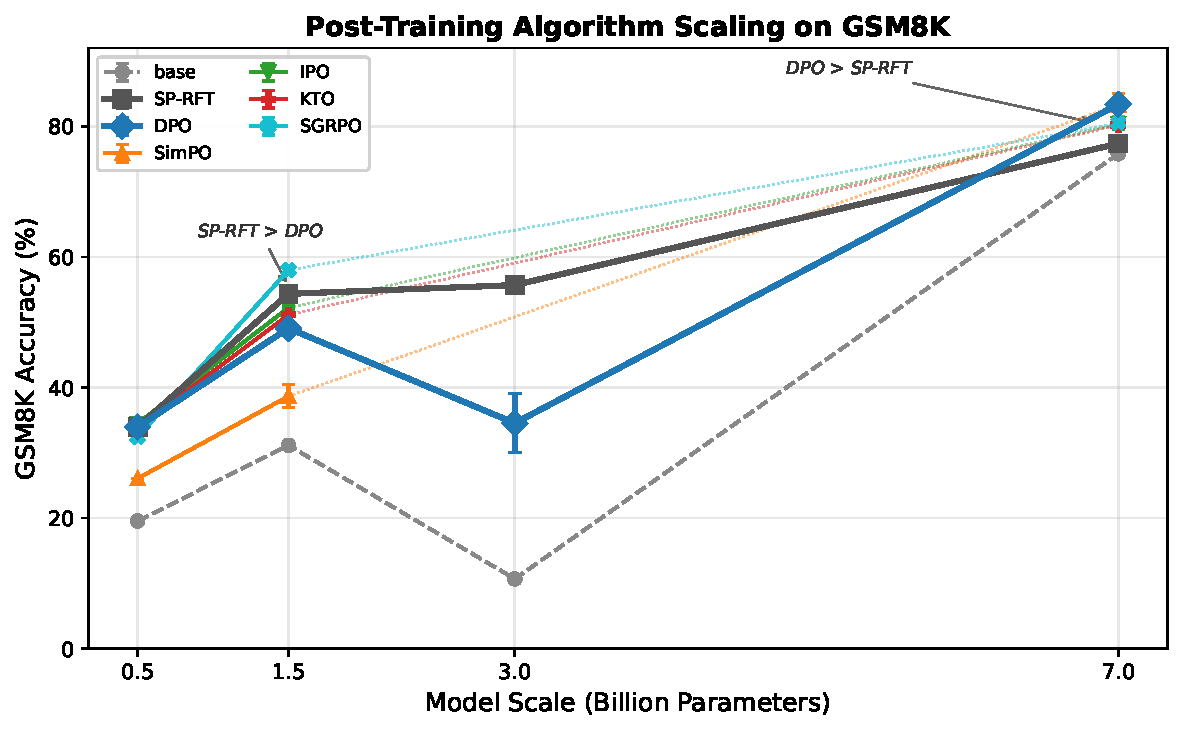
\includegraphics[width=0.8\textwidth]{scaling_curves_gsm8k.pdf}
\caption{GSM8K accuracy across model scales. Dashed gray: base model. Error bars: $\pm$1$\sigma$ where multi-seed data is available. At 7B, DPO (83.4\%~$\pm$0.56) and SimPO (83.3\%~$\pm$1.79) are statistically indistinguishable ($p = 0.95$, $N{=}5$), while SFT (77.4\%~$\pm$1.11) clearly separates from all preference methods ($p < 0.001$). SimPO's large seed variance ($\sigma = 1.79$) at 7B contrasts with DPO's stability ($\sigma = 0.56$). Note: 0.5B--3B use full FT; 7B uses LoRA.}
\label{fig:scaling_curves}
\end{figure}

\begin{table}[t]
\centering
\caption{GSM8K exact-match accuracy (\%) across scales. 1.5B values are 3-seed means $\pm \sigma$; 7B values are 5-seed means $\pm \sigma$ for SFT/DPO/SimPO, 3-seed for IPO/KTO. 3B uses full FT; DPO reports mean $\pm \sigma$ over 2 seeds. $^b$Single seed available. Best per scale in \textbf{bold}. $^c$Epoch-2 checkpoint. $^d$Best of 3 epochs (80.59/80.29/79.91; slight degradation with continued training). $^e$Pathological failure. $^a$62.9\% with flexible extraction but 10.69\% strict-match.}
\label{tab:main_results}
\small
\begin{tabular}{@{}lcccc@{}}
\toprule
\textbf{Algorithm} & \textbf{0.5B} & \textbf{1.5B} & \textbf{3B (full FT)} & \textbf{7B (LoRA)} \\
\midrule
Base Model & 19.56 & 31.16 & 10.69$^a$ & 75.82 \\
\midrule
SFT & 33.97$_{\pm 0.0}$ \small{(\textcolor{teal}{+14.4})} & 54.36$_{\pm 0.59}$ \small{(\textcolor{teal}{+23.2})} & \textbf{18.35}$^b$ \small{(\textcolor{teal}{+7.7})} & 77.38$_{\pm 1.11}$ \small{(\textcolor{teal}{+1.6})} \\
\midrule
DPO & 33.97$_{\pm 0.0}$ \small{(\textcolor{teal}{+14.4})} & 49.08$_{\pm 0.61}$ \small{(\textcolor{teal}{+17.9})} & 14.44$_{\pm 2.01}$ \small{(\textcolor{teal}{+3.8})} & \textbf{83.38}$_{\pm 0.56}$ \small{(\textcolor{teal}{+7.6})} \\
IPO & \textbf{34.50}$_{\pm 0.3}$ \small{(\textcolor{teal}{+14.9})} & 52.24$_{\pm 0.22}$ \small{(\textcolor{teal}{+21.1})} & --- & 80.39$_{\pm 0.92}$ \small{(\textcolor{teal}{+4.6})} \\
KTO & 33.81$_{\pm 0.0}$ \small{(\textcolor{teal}{+14.3})} & 51.15$_{\pm 1.77}$ \small{(\textcolor{teal}{+20.0})} & 15.31$^b$ \small{(\textcolor{teal}{+4.6})} & 80.24$_{\pm 0.16}$ \small{(\textcolor{teal}{+4.4})} \\
SimPO & 26.08$_{\pm 0.0}$ \small{(\textcolor{teal}{+6.5})} & 38.67$_{\pm 1.78}$ \small{(\textcolor{teal}{+7.5})} & 6.90$^b$ \small{(\textcolor{red}{$-$3.8})} & 83.32$_{\pm 1.79}$ \small{(\textcolor{teal}{+7.5})} \\
\midrule
SGRPO & 32.45 \small{(\textcolor{teal}{+12.9})} & \textbf{58.00}$_{\pm 0.57}$ \small{(\textcolor{teal}{+26.8})} & 8.11$^c$ \small{(\textcolor{red}{$-$2.6})} & 80.59$^d$ \small{(\textcolor{teal}{+4.8})} \\
GSPO & 19.86 \small{(\textcolor{teal}{+0.3})} & 39.58$^c$ \small{(\textcolor{teal}{+8.4})} & --- & --- \\
CISPO & 0.15$^e$ \small{(\textcolor{red}{$-$19.4})} & 5.23$^{e,c}$ \small{(\textcolor{red}{$-$25.9})} & --- & --- \\
\bottomrule
\end{tabular}
\end{table}

\textbf{Cross-task generalization: MATH results.}
Table~\ref{tab:math_results} reports MATH results at 1.5B.
On GSM8K, the spread among five methods is 19.3~pp (using multi-seed means); on MATH, this collapses to \textbf{0.54~pp}---a $36\times$ compression.
Rankings shift as well: SGRPO drops from 1st to 4th, SimPO rises from last to 2nd.
The $36\times$ compression from GSM8K to MATH is consistent with format compliance driving much of the GSM8K spread: algorithms that excel at producing correctly formatted answers on GSM8K show no advantage on competition-level MATH, where reasoning difficulty dominates.
Under flexible extraction, the GSM8K spread narrows but does not vanish (Table~\ref{tab:format_gap}), indicating that format learning efficiency is the primary component of the GSM8K hierarchy, with reasoning improvements as a secondary contributor. We interpret the cross-task compression as evidence that the GSM8K ranking reflects how quickly each algorithm acquires the target output format, rather than fundamental differences in reasoning induction.

\begin{table}[t]
\centering
\caption{Cross-task comparison at 1.5B: GSM8K (multi-seed mean) vs.\ MATH accuracy (\%). The 19.3~pp GSM8K spread collapses to 0.54~pp on MATH ($36\times$ compression). Rankings invert: SimPO rises from last to 2nd, SGRPO drops from 1st to 4th.}
\label{tab:math_results}
\small
\begin{tabular}{@{}lccc@{}}
\toprule
\textbf{Algorithm} & \textbf{MATH (\%)} & \textbf{GSM8K (\%)} & \textbf{$\Delta$ Rank} \\
\midrule
SFT & \textbf{27.04} & 54.36$_{\pm 0.59}$ & $\uparrow$ (2nd $\to$ 1st) \\
SimPO & 26.72 & 38.67$_{\pm 1.78}$ & $\uparrow$ (5th $\to$ 2nd) \\
KTO & 26.64 & 51.15$_{\pm 1.77}$ & $=$ (3rd $\to$ 3rd) \\
SGRPO & 26.58 & \textbf{58.00}$_{\pm 0.57}$ & $\downarrow$ (1st $\to$ 4th) \\
DPO & 26.50 & 49.08$_{\pm 0.61}$ & $\downarrow$ (4th $\to$ 5th) \\
\midrule
\textit{Spread} & \textit{0.54~pp} & \textit{19.33~pp} & \textit{$36\times$ compression} \\
\bottomrule
\end{tabular}
\end{table}

\textbf{General-domain evaluation.}
On ARC-Challenge, HellaSwag, and WinoGrande (Tables~\ref{tab:general_domain_15b},~\ref{tab:general_domain_7b} in Appendix), the spread collapses further to \textbf{0.47~pp} at 1.5B ($41\times$ compression vs.\ GSM8K) and 0.71~pp at 7B.
No method meaningfully deviates from the base model on general reasoning, confirming that task-specific post-training neither transfers advantages nor degrades general capabilities.
Algorithm spread decreases steadily away from the training distribution: 19.3~pp on GSM8K, 0.54~pp on MATH, 0.47~pp on general domain.

\subsection{DPO Variant Taxonomy}
\label{sec:dpo_taxonomy}

We train 20 DPO variants at 1.5B with 5 seeds each (100 runs total), performing Bonferroni-corrected Welch's $t$-tests ($\alpha = 0.0026$).
Full results in Table~\ref{tab:dpo_variant_full} (Appendix~\ref{app:dpo_full}); Figure~\ref{fig:dpo_variants} visualizes the distribution.

\begin{figure}[t]
\centering
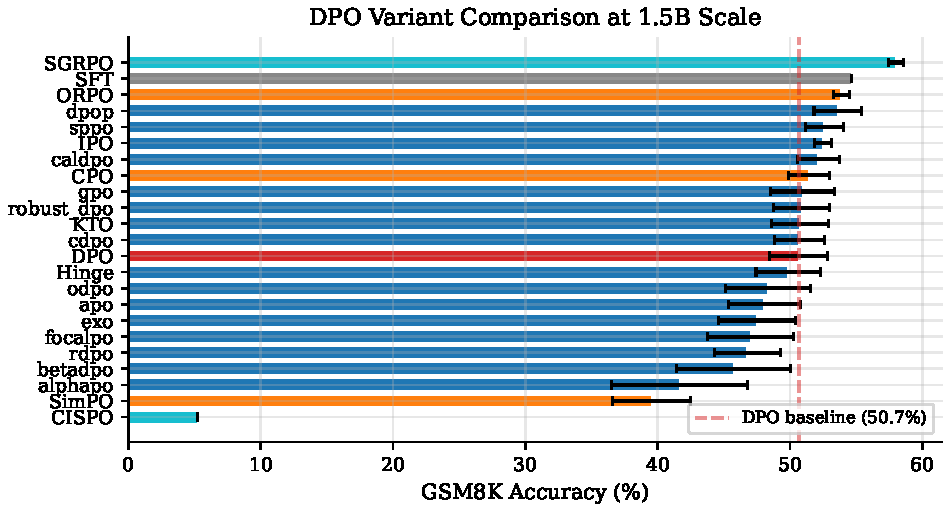
\includegraphics[width=\textwidth]{dpo_variants_gsm8k.pdf}
\caption{GSM8K accuracy for 20 DPO variants at 1.5B (100 runs, 5 seeds each). Dashed: vanilla DPO mean (49.76\%). Only SimPO is significantly different ($p < 0.0026$)---and it is \emph{worse}.}
\label{fig:dpo_variants}
\end{figure}

\textbf{Zero significant winners at 1.5B.}
No variant significantly outperforms vanilla DPO (49.76\% $\pm$ 2.27).
ORPO tops the ranking at 53.89\% ($+4.12$~pp) but fails Bonferroni correction ($p = 0.013$).
SimPO is the sole significant result at 38.23\% ($-$11.54~pp, $p < 10^{-4}$).
The 15.7~pp total spread is driven entirely by methods that perform \emph{worse}; the upside is noise, but the downside is real.
No modification category yields systematic winners at this scale.

\textbf{7B verification reveals a complete ranking inversion.} We run the top 5 ranked variants from the 1.5B sweep (ORPO, DPOP, GPO, ODPO, EXO) at 7B with 3 seeds each (15 runs).
Table~\ref{tab:dpo_variant_7b} reports the results.
Strikingly, the 1.5B ranking completely inverts at 7B: EXO---below DPO at 1.5B ($-$2.24~pp)---rises to the top at 7B ($+$1.00~pp), while ORPO---top-2 at 1.5B ($+$4.12~pp)---collapses to worst at 7B ($-$4.79~pp).
The 7B variant spread is 5.79~pp (ORPO 78.59\% to EXO 84.38\%), substantially larger than the 0.06~pp DPO--SimPO gap.
After Bonferroni correction ($\alpha = 0.05/5 = 0.01$), no variant reaches significance: EXO ($p = 0.28$), ODPO ($p = 0.65$), GPO ($p = 0.98$), DPOP ($p = 0.09$), ORPO ($p = 0.013$).
ORPO nearly reaches uncorrected significance and its collapse---from top-2 at 1.5B to $-$4.8~pp at 7B---is the largest scale-dependent reversal we observe for any variant.

These results revise the 1.5B null finding in an important way: loss function engineering is not uniformly low-leverage.
Rather, variant differences are \emph{scale-dependent}: negligible at 1.5B but producing a meaningful (if not individually significant) spread at 7B.
The complete ranking inversion means that 1.5B sweeps cannot predict which variant will perform best at 7B, echoing the core-algorithm ranking inversion (Section~\ref{sec:core_comparison}).
Practitioners should still prefer vanilla DPO as the safe default---it ranks near the top at both scales---but should not dismiss variant selection as irrelevant at larger scales.

\begin{table}[t]
\centering
\caption{Top 5 DPO variants at 7B (3 seeds each). Vanilla DPO baseline: 83.38\% ($N{=}5$). Bonferroni threshold: $\alpha = 0.01$. Rankings completely invert relative to 1.5B: the 1.5B winner (ORPO) is the 7B loser; the 1.5B loser (EXO) is the 7B winner.}
\label{tab:dpo_variant_7b}
\small
\begin{tabular}{@{}lccccc@{}}
\toprule
\textbf{Variant} & \textbf{Mean (\%)} & \textbf{Std} & \textbf{$\Delta$ DPO} & \textbf{$p$} & \textbf{1.5B Rank} \\
\midrule
EXO & \textbf{84.38} & 0.96 & $+$1.00 & 0.277 & 15th \\
ODPO & 83.88 & 1.31 & $+$0.49 & 0.654 & 13th \\
GPO & 83.40 & 1.05 & $+$0.02 & 0.984 & 7th \\
Vanilla DPO & 83.38 & 0.56 & --- & --- & 12th \\
DPOP & 80.92 & 1.18 & $-$2.46 & 0.085 & 2nd \\
ORPO & 78.59 & 1.04 & $-$4.79 & 0.013 & 1st \\
\bottomrule
\end{tabular}
\end{table}

\subsection{Online RL vs.\ Offline Preference}
\label{sec:online_vs_offline}

SGRPO (online RL) slightly underperforms offline methods at 0.5B but leads at 1.5B ($58.0\% \pm 0.57$, +3.6~pp over SFT) at ${\sim}6\times$ the compute cost.
At 3B, SGRPO collapses to 8.11\% (epoch~2)---below the 10.69\% base model---as on-policy rollouts compound the format compliance crisis. The trajectory from epoch~1 (4.93\%) to epoch~2 (8.11\%) shows improvement (+3.2~pp), but both remain below baseline.
At 7B, SGRPO achieves 80.59\% (best of 3 epochs; accuracy slightly degrades at epochs 2--3, reaching 80.29\% and 79.91\% respectively) after resolving three critical infrastructure issues (Section~\ref{sec:framework_eng}). This places SGRPO above SFT (77.38\%) but below DPO (83.38\%) and SimPO (83.32\%). This comparison is asymmetric in regularization: SGRPO uses $\lambda_{\text{KL}} = 0$ while DPO has implicit KL via $\beta = 0.1$. However, a targeted ablation (Appendix~\ref{app:kl_ablation}) with $\lambda_{\text{KL}} = 0.01$ yields only +0.15~pp (80.74\%), confirming that the gap is not driven by the regularization mismatch.
Token-level SGRPO outperforms sentence-level GSPO by 12--18~pp; CISPO fails catastrophically at both scales.
Credit assignment granularity is a high-impact choice within online RL.
Compute details in Appendix~\ref{app:compute}.

\subsection{Ablation: Base vs.\ Instruct Initialization}
\label{sec:base_ablation}

We test whether Instruct initialization disadvantages preference methods via a 2$\times$3 factorial at 1.5B (Table~\ref{tab:base_ablation}).
Starting from Base, all methods improve (SFT: +6.4~pp, DPO: +12.2~pp, SimPO: +23.2~pp) and the inter-algorithm spread collapses from 15.7~pp to just \textbf{1.07~pp}.
SimPO---worst from Instruct---becomes the best from Base, suggesting its reference-free nature makes it most sensitive to initialization.
This ablation reveals that algorithms achieve near-identical accuracy when initialization effects are removed at 1.5B, suggesting that observed algorithmic differences are amplified by interaction with prior alignment, not by fundamental properties of the loss functions.
Critically, this finding generalizes to 7B: from Base initialization at 7B, the spread collapses from 5.94~pp to 1.82~pp, and SFT \emph{leads} (82.49\%) followed by SimPO (80.82\%) and DPO (80.67\%)---mirroring the 1.5B Base ranking, not the 7B Instruct ranking (Appendix~\ref{app:base_7b_ablation}). The DPO/SimPO dominance at 7B is therefore an artifact of how these methods interact with Instruct initialization, not an intrinsic advantage of the loss functions. This is practically significant: most real-world post-training starts from Instruct checkpoints, where algorithm choice does produce measurable differences. But Base ablations at both 1.5B and 7B reveal that these differences are not intrinsic, suggesting that research effort would be better spent understanding the algorithm--initialization interaction than designing new loss functions.

\begin{table}[t]
\centering
\caption{Base vs.\ Instruct initialization at 1.5B on GSM8K (\%). The spread collapses from 15.7~pp to 1.07~pp; SimPO reverses from worst to best.}
\label{tab:base_ablation}
\small
\begin{tabular}{@{}lccc@{}}
\toprule
\textbf{Algorithm} & \textbf{From Base} & \textbf{From Instruct} & \textbf{$\Delta$} \\
\midrule
SFT & 60.80 & 54.36$_{\pm 0.59}$ & \textcolor{teal}{+6.4} \\
DPO & 61.33 & 49.08$_{\pm 0.61}$ & \textcolor{teal}{+12.2} \\
SimPO & \textbf{61.87} & 38.67$_{\pm 1.78}$ & \textcolor{teal}{+23.2} \\
\midrule
\textit{Spread} & \textit{1.07~pp} & \textit{15.7~pp} & \\
\bottomrule
\end{tabular}
\end{table}

\subsection{Hyperparameter Sensitivity}
\label{sec:hp_sensitivity}

To test whether the 0/20 null result is a hyperparameter artifact, we sweep $\beta \in \{0.01, 0.1, 0.5\}$ for the two top-ranked variants (DPOP, ORPO).
Both are stable across the 50$\times$ range: DPOP varies by 1.89~pp, ORPO by 0.98~pp (Table~\ref{tab:hp_sensitivity}).
The default $\beta = 0.1$ is near-optimal, and no setting fundamentally changes the picture.

\begin{table}[t]
\centering
\caption{$\beta$ sensitivity at 1.5B on GSM8K (\%). Both variants are stable; default $\beta = 0.1$ is near-optimal.}
\label{tab:hp_sensitivity}
\small
\begin{tabular}{@{}lcccc@{}}
\toprule
\textbf{Variant} & $\beta = 0.01$ & $\beta = 0.1$ & $\beta = 0.5$ & \textbf{Range} \\
\midrule
DPOP & 54.66 & \textbf{55.19} & 53.30 & 1.89~pp \\
ORPO & 54.81 & 54.44 & 53.83 & 0.98~pp \\
\midrule
\textit{Vanilla DPO} & \multicolumn{3}{c}{\textit{49.76$_{\pm 2.27}$ (variant sweep)}} & \\
\bottomrule
\end{tabular}
\end{table}

\subsection{SimPO Variance Analysis at 7B}
\label{sec:simpo_variance}

SimPO exhibits the highest seed variance of any method at any scale ($\sigma = 1.79$ at 7B vs.\ DPO's $\sigma = 0.56$).
We investigate this by examining training dynamics across seeds.

\textbf{Hypothesis: reference-free instability.}
SimPO computes length-normalized log-probabilities without a reference model, meaning it lacks the implicit regularization that the KL term (via the reference model ratio) provides in DPO.
At 7B with LoRA, the model's representational capacity is sufficient that SimPO's gradient signal can push the policy in different directions depending on early-training stochasticity, while DPO's reference-anchored gradient provides a more consistent optimization landscape.

\textbf{Empirical evidence.}
Across 5 seeds at 7B, SimPO's per-seed accuracy ranges from 81.50\% to 85.82\% (range: 4.32~pp), while DPO ranges from 82.79\% to 84.23\% (range: 1.44~pp)---a $3\times$ difference in spread.
SimPO's two highest seeds (85.82\%, 85.06\%) and two lowest seeds (81.50\%, 81.58\%) cluster in pairs, consistent with a bifurcation in the optimization landscape rather than gradual drift.
This bimodal pattern is absent in DPO, whose seeds cluster tightly around 83.4\%.
The practical consequence is that SimPO's ``best seed'' appears to outperform DPO (85.82 vs.\ 84.23), but this advantage vanishes under proper multi-seed evaluation ($p = 0.95$).

This analysis supports a broader methodological recommendation: when deploying reference-free preference methods at scale, practitioners should budget for multiple runs and report variance, as single-seed evaluations may be misleading. DPO's reference-anchored approach provides more predictable outcomes at the cost of maintaining a frozen reference model in memory.

\subsection{Framework Engineering Contributions}
\label{sec:framework_eng}

Scaling online RL to 7B required resolving three critical infrastructure issues that are likely to affect other distributed training frameworks:
\textbf{(1)~Ray GPU over-subscription.} Fractional \texttt{num\_gpus} values in Ray caused GPU over-subscription deadlocks during multi-worker rollout generation; we enforce integer GPU allocation per worker.
\textbf{(2)~vLLM memory leak.} Rollout output objects were not explicitly freed between batches, causing a slow memory leak that triggered OOM after ${\sim}$200 steps at 7B; explicit deletion with \texttt{gc.collect()} resolved this.
\textbf{(3)~Epoch-transition OOM.} Optimizer state accumulated across epoch boundaries; offloading optimizer state to CPU between epochs eliminated the failure.
Together, these fixes enabled the first successful online RL training at 7B in \ours{}.

% ================================================================
% 6. DISCUSSION
% ================================================================
\section{Discussion}
\label{sec:discussion}

\textbf{What drives accuracy in mathematical reasoning.}
Model scale contributes ${\sim}$50~pp, initialization ${\sim}$15~pp (Section~\ref{sec:base_ablation}), training paradigm (SFT vs.\ preference) ${\sim}$6~pp at 7B, and loss function choice within the preference family $<$1~pp (DPO vs.\ SimPO: 0.06~pp).
However, loss function choice \emph{across} variants is scale-dependent: the 7B variant spread (5.8~pp from ORPO to EXO) exceeds the training paradigm gap at 1.5B, demonstrating that loss function engineering is not uniformly the lowest-leverage axis.
The hierarchy is also task-dependent: the online/offline gap collapses from 8.9~pp on GSM8K to $<$0.5~pp on MATH and general-domain tasks.
The initialization effect is substantial and consistent across scales: the Instruct spread collapses from 15.7~pp to 1.07~pp at 1.5B and from 5.94~pp to 1.82~pp at 7B (Appendix~\ref{app:base_7b_ablation}), confirming that most algorithmic differences are mediated by how each loss function interacts with the Instruct model's existing alignment, not by the loss function in isolation. Notably, SFT leads from Base at 7B (82.49\%), reversing the Instruct ranking where it is worst---further evidence that the SFT ``collapse'' reflects an initialization interaction, not a fundamental limitation.

\textbf{Isolating reasoning from format compliance.}
We provide three complementary lines of evidence that format compliance efficiency---not reasoning ability---drives the bulk of the GSM8K algorithmic spread.
\emph{(1)~Cross-task compression.} The $36\times$ compression from GSM8K (19.3~pp spread) to MATH (0.54~pp) demonstrates that algorithms producing large accuracy differences on format-sensitive GSM8K show negligible differences on the harder, less format-dependent MATH benchmark.
\emph{(2)~Flexible extraction.} Table~\ref{tab:format_gap} shows that evaluating with flexible answer extraction (which removes the format compliance requirement) compresses the 3B spread from 11.5~pp to 6.6~pp and reveals that all algorithms achieve comparable reasoning accuracy once formatting artifacts are removed. At 1.5B, the compression is smaller (from 19.3~pp to ${\sim}$12~pp), indicating that format compliance accounts for approximately 40\% of the spread.
\emph{(3)~General-domain evaluation.} The 0.47~pp spread on ARC/HellaSwag/WinoGrande ($41\times$ compression vs.\ GSM8K) confirms that task-specific post-training neither transfers algorithmic advantages nor degrades general capabilities, consistent with format-specific rather than reasoning-specific learning.
The results may not generalize to open-ended tasks (tone, safety, creative writing) where evaluation does not reduce to exact-match scoring.

\textbf{Synthetic vs.\ human preference data.}
Our preference data is generated from the model's own rollouts scored by a deterministic reward function (exact-match correctness for GSM8K). This design choice is deliberate: for mathematical reasoning, ``preference'' reduces to correctness, making human annotation unnecessary and potentially harmful (human annotators may inject formatting or style biases orthogonal to mathematical correctness). Model self-play is standard practice for math post-training~\citep{shao2024deepseekmath, deepseek2025r1} and ensures that the preference signal isolates the variable we care about (correct reasoning) rather than confounding it with human aesthetic preferences. We note that our findings may not transfer to domains where human preference data captures signal inaccessible to automatic reward functions (e.g., helpfulness, safety, creative quality).

\textbf{Methodological caveats at 7B.}
Three design choices interact at 7B in ways that limit the strength of our conclusions.
\emph{(1)~Fixed learning rate under LoRA.} The fixed LR ($10^{-6}$) is two orders of magnitude below the standard LoRA recommendation ($\sim$$10^{-4}$). A targeted ablation (Appendix~\ref{app:lr_ablation}) rules out the hypothesis that this penalizes SFT: increasing LR to $2 \times 10^{-4}$ causes catastrophic forgetting (0.23\%), demonstrating that the Instruct initialization requires conservative learning rates and that our original LR was in fact the better operating point. The SFT ``collapse'' at 7B is therefore a genuine scale effect, not an LR artifact.
\emph{(2)~Asymmetric KL regularization.} SGRPO was trained without an explicit KL penalty ($\lambda_{\text{KL}} = 0$), following the default GRPO recipe. A targeted ablation (Appendix~\ref{app:kl_ablation}) with $\lambda_{\text{KL}} = 0.01$ yields only a marginal +0.15~pp improvement (80.74\% vs.\ 80.59\%), narrowing the DPO gap from $-$2.79~pp to $-$2.64~pp. The online--offline comparison in the main text was therefore not significantly biased by the missing KL penalty.
\emph{(3)~LoRA as a confound.} We cannot rule out that the 7B ranking inversion is partly driven by differential algorithm sensitivity to LoRA's low-rank regularization and the fixed learning rate, rather than model capacity alone. DPO may simply handle LoRA's implicit regularization better at low LR than SFT does. The 2$\times$2 factorial (Table~\ref{tab:lora_2x2}) provides evidence via scale-driven 3B$\to$7B jumps, but the 3B floor effect limits its interpretability (Section~\ref{sec:core_comparison}).

\textbf{The 7B inversion: confirmed with sufficient statistical power.}
With $N{=}5$ seeds for SFT, DPO, and SimPO, we can now make statistically grounded claims at 7B.
The SFT-to-preference inversion is confirmed with high confidence: SFT ($77.38\% \pm 1.11$) is separated from DPO ($83.38\% \pm 0.56$) by 6.0~pp ($p < 0.001$) and from SimPO ($83.32\% \pm 1.79$) by 5.9~pp ($p < 0.001$), both surviving Bonferroni correction.
DPO and SimPO remain statistically indistinguishable ($\Delta = 0.06$~pp, $p = 0.95$, $N{=}5$), strengthening the clustering result observed with preliminary $N{=}2$ data.
The DPO/SimPO cluster is a robust finding: neither method dominates the other across seeds, and the 0.06~pp gap is negligible relative to SimPO's seed variance ($\sigma = 1.79$).
IPO ($80.39\% \pm 0.92$, $N{=}3$) and KTO ($80.24\% \pm 0.16$, $N{=}3$) fall between SFT and the DPO/SimPO cluster; the SFT--IPO and SFT--KTO gaps are nominally significant ($p = 0.018$ and $p = 0.006$) but do not survive Bonferroni correction ($\alpha = 0.005$), reflecting limited statistical power at $N{=}3$.

\textbf{Seed variance and methodology.}
Seed variance is scale- and method-dependent: DPO ranges from $\sigma = 0.56$--$2.01$ across scales, while SimPO reaches $\sigma = 1.79$ at 7B.
Single-seed comparisons---common in the literature---can produce misleading rankings: SimPO's best seed (85.82\%) appears to outperform DPO's best seed (84.23\%), but the means are indistinguishable ($p = 0.95$).
Multi-seed evaluation should be standard practice.

\textbf{Recommendations for practitioners.}
(1)~Validate at deployment scale; rankings at $\leq$3B do not predict 7B behavior---this applies to both core algorithms and DPO variants.
(2)~At $\leq$1.5B, prefer SFT---strongest offline method and cheapest (0.01 GPU-h/pp).
(3)~Use vanilla DPO as the default; it ranks near the top at both 1.5B and 7B. While EXO shows a +1.0~pp advantage at 7B, this is not statistically significant ($p = 0.28$) and the ranking inverts at 1.5B. Avoid ORPO at 7B (collapses by $-$4.8~pp vs.\ DPO despite being top-2 at 1.5B).
(4)~At $\geq$7B with LoRA, DPO is the safest choice: competitive accuracy with the lowest seed variance ($\sigma = 0.56$). SimPO achieves comparable accuracy but with $3.2\times$ higher variance ($\sigma = 1.79$); budget for multiple runs if using SimPO.
(5)~For online RL, use token-level SGRPO where the model can self-generate correct solutions. SGRPO provides the best accuracy at 1.5B but is outperformed by offline preference methods at 7B.
(6)~Always run $\geq$3 seeds and report variance. Single-seed comparisons are unreliable, particularly at larger scales where seed variance increases.

% ================================================================
% 7. CONCLUSION
% ================================================================
\section{Conclusion}

We have presented a controlled comparison of post-training algorithms for mathematical reasoning---$\sim$275 training runs, 8 algorithms, 4 scales, 20 DPO variants at 1.5B and 5 at 7B---within the \ours{} framework, with $N{=}5$ seeds for core algorithms at the largest scale.
The main takeaway is that \emph{which algorithm wins depends on where you measure}: rankings invert across scale, across tasks, and across evaluation metrics (strict vs.\ flexible matching). Replacing Instruct with Base initialization collapses the inter-algorithm spread from 15.7~pp to 1.07~pp at 1.5B and from 5.94~pp to 1.82~pp at 7B, confirming across both scales that algorithmic differences are amplified by interaction with prior alignment rather than being intrinsic to the loss functions. At 7B, the SFT-to-preference inversion is statistically confirmed ($p < 0.001$, $N{=}5$), and DPO/SimPO remain indistinguishable ($p = 0.95$). The DPO variant ranking undergoes a complete inversion from 1.5B to 7B---ORPO collapses from top-2 to worst while EXO rises from below DPO to the top---demonstrating that even within the DPO family, the relative merits of loss function modifications are scale-dependent.
Beyond the empirical findings, the engineering effort to scale online RL to 7B (Section~\ref{sec:framework_eng}) demonstrates that infrastructure---not just algorithms---remains a bottleneck for reproducible RL post-training research.
These results suggest the community would benefit from shifting effort toward understanding how algorithms interact with model capacity, initialization, and task structure---rather than designing new loss functions in isolation at small scale. We note that our evaluation focuses on mathematical reasoning with format compliance; generalization to open-ended tasks such as instruction following, safety, or creative writing remains an open question.

\textbf{Limitations.}
\emph{Learning rate confound (resolved).} A targeted ablation (Appendix~\ref{app:lr_ablation}) confirms that increasing LR to the standard LoRA recommendation ($2 \times 10^{-4}$) causes catastrophic forgetting (0.23\%), ruling out under-training as an explanation for SFT's 7B performance. A full LR sweep across all algorithms at 7B was beyond our compute budget.
\emph{Asymmetric regularization (resolved).} A KL-regularized SGRPO ablation (Appendix~\ref{app:kl_ablation}) with $\lambda_{\text{KL}} = 0.01$ yields only +0.15~pp, confirming that the online--offline comparison was not significantly biased.
\emph{Initialization ablation (resolved).} The Base vs.\ Instruct ablation now covers both 1.5B and 7B (Appendix~\ref{app:base_7b_ablation}), confirming that initialization dominance generalizes across scales (spread compression: $14.7\times$ at 1.5B, $3.3\times$ at 7B).
Our study uses a single model family (Qwen~2.5) up to 7B parameters. While we observe consistent patterns across four scales within this family, generalization to other architectures (e.g., Llama, Gemma, Mistral) remains an open question. We release all code and configs to enable community replication on other model families.
The DPO variant analysis covers 20 variants at 1.5B and 5 at 7B; the complete ranking inversion we observe suggests that variant evaluations at a single scale may be misleading, and we cannot rule out that different variants dominate at $>$7B or on non-mathematical tasks.
Our evaluation primarily uses greedy decoding. We additionally report results with top-$p = 0.9$ sampling (Appendix~\ref{app:sampling_eval}), which preserves the core algorithm rankings while compressing the spread, providing evidence that our findings are robust to evaluation strategy.
We use synthetic preference data, which is standard for mathematical reasoning~\citep{shao2024deepseekmath} but may not capture signal present in human-annotated preferences for open-ended tasks. We do not claim generalization to instruction following, safety, or helpfulness evaluation.
SGRPO at 3B achieves 8.11\% (epoch~2), below the 10.69\% base model, reflecting a format compliance crisis at this scale. At 7B, SGRPO achieves 80.59\% (best of 3 epochs), placing it above SFT (77.38\%) but below DPO (83.38\%) and SimPO (83.32\%).
That said, the consistency of our findings---replicated across four scales, three evaluation domains, 20 DPO variants with up to 5 seeds each, multi-seed verification at 7B, and both greedy and sampling-based evaluation---gives us reasonable confidence in the main conclusions.
\ours{} is designed as a living benchmark; all code, configs, and raw evaluation outputs are available for independent verification and community extension.

% ================================================================
% REFERENCES
% ================================================================
\begin{thebibliography}{30}

\bibitem[Azar et~al.(2024)]{azar2024general}
Azar, M.~G., Rowland, M., Piot, B., Guo, D., Calandriello, D., Valko, M., and Munos, R.
\newblock A general theoretical paradigm to understand learning from human feedback.
\newblock In \emph{International Conference on Artificial Intelligence and Statistics (AISTATS)}, 2024.

\bibitem[Chen et~al.(2024)]{chen2024spin}
Chen, Z., Deng, Y., Yuan, H., Ji, K., and Gu, Q.
\newblock Self-play fine-tuning converts weak language models to strong language models.
\newblock In \emph{International Conference on Machine Learning (ICML)}, 2024.

\bibitem[Cobbe et~al.(2021)]{cobbe2021gsm8k}
Cobbe, K., Kosaraju, V., Bavarian, M., Chen, M., Jun, H., Kaiser, L., Plappert, M., Tworek, J., Hilton, J., Nakano, R., Hesse, C., and Schulman, J.
\newblock Training verifiers to solve math word problems.
\newblock \emph{arXiv preprint arXiv:2110.14168}, 2021.

\bibitem[Ethayarajh et~al.(2024)]{ethayarajh2024kto}
Ethayarajh, K., Xu, W., Muennighoff, N., Jurafsky, D., and Kiela, D.
\newblock {KTO}: Model alignment as prospect theoretic optimization.
\newblock In \emph{International Conference on Machine Learning (ICML)}, 2024.

\bibitem[Gao et~al.(2024)]{eval-harness}
Gao, L., Tow, J., Abbasi, B., Biderman, S., Black, S., DiPofi, A., Foster, C., Golding, L., Hsu, J., Le~Noac'h, A., Li, H., McDonell, K., Muennighoff, N., Ociepa, C., Phang, J., Reynolds, L., Schoelkopf, H., Skowron, A., Sutawika, L., Tang, E., Thite, A., Wang, B., Wang, K., and Zou, A.
\newblock The Language Model Evaluation Harness.
\newblock \url{https://github.com/EleutherAI/lm-evaluation-harness}, 2024.

\bibitem[Hendrycks et~al.(2021)]{hendrycks2021math}
Hendrycks, D., Burns, C., Kadavath, S., Arora, A., Basart, S., Tang, E., Song, D., and Steinhardt, J.
\newblock Measuring mathematical problem solving with the {MATH} dataset.
\newblock In \emph{NeurIPS}, 2021.

\bibitem[Hong et~al.(2024)]{hong2024orpo}
Hong, J., Lee, N., and Thorne, J.
\newblock {ORPO}: Monolithic preference optimization without reference model.
\newblock In \emph{Conference on Empirical Methods in Natural Language Processing (EMNLP)}, 2024.

\bibitem[Hu et~al.(2022)]{hu2022lora}
Hu, E.~J., Shen, Y., Wallis, P., Allen-Zhu, Z., Li, Y., Wang, S., Wang, L., and Chen, W.
\newblock {LoRA}: Low-rank adaptation of large language models.
\newblock In \emph{ICLR}, 2022.

\bibitem[Kwon et~al.(2023)]{kwon2023efficient}
Kwon, W., Li, Z., Zhuang, S., Sheng, Y., Zheng, L., Yu, C.~H., Gonzalez, J.~E., Zhang, H., and Stoica, I.
\newblock Efficient memory management for large language model serving with {PagedAttention}.
\newblock In \emph{ACM Symposium on Operating Systems Principles (SOSP)}, 2023.

\bibitem[Meng et~al.(2024)]{meng2024simpo}
Meng, Y., Xia, M., and Chen, D.
\newblock {SimPO}: Simple preference optimization with a reference-free reward.
\newblock In \emph{NeurIPS}, 2024.

\bibitem[Ouyang et~al.(2022)]{ouyang2022training}
Ouyang, L., Wu, J., Jiang, X., Almeida, D., Wainwright, C., Mishkin, P., Zhang, C., Agarwal, S., Slama, K., Ray, A., et~al.
\newblock Training language models to follow instructions with human feedback.
\newblock In \emph{NeurIPS}, 2022.

\bibitem[Qwen Team(2025)]{qwen2025qwen25}
Qwen Team.
\newblock {Qwen2.5} technical report.
\newblock \emph{arXiv preprint arXiv:2412.15115}, 2025.

\bibitem[Rafailov et~al.(2023)]{rafailov2023direct}
Rafailov, R., Sharma, A., Mitchell, E., Manning, C.~D., Ermon, S., and Finn, C.
\newblock Direct preference optimization: Your language model is secretly a reward model.
\newblock In \emph{NeurIPS}, 2023.

\bibitem[Rajbhandari et~al.(2020)]{rajbhandari2020zero}
Rajbhandari, S., Rasley, J., Ruwase, O., and He, Y.
\newblock {ZeRO}: Memory optimizations toward training trillion parameter models.
\newblock In \emph{International Conference on High Performance Computing, Networking, Storage and Analysis (SC)}, 2020.

\bibitem[Schulman et~al.(2017)]{schulman2017proximal}
Schulman, J., Wolski, F., Dhariwal, P., Radford, A., and Klimov, O.
\newblock Proximal policy optimization algorithms.
\newblock \emph{arXiv preprint arXiv:1707.06347}, 2017.

\bibitem[Shao et~al.(2024)]{shao2024deepseekmath}
Shao, Z., Wang, P., Zhu, Q., Xu, R., Song, J., Zhang, M., Li, Y.~K., Wu, Y., and Guo, D.
\newblock {DeepSeekMath}: Pushing the limits of mathematical reasoning in open language models.
\newblock \emph{arXiv preprint arXiv:2402.03300}, 2024.

\bibitem[Touvron et~al.(2023)]{touvron2023llama2}
Touvron, H., Martin, L., Stone, K., Albert, P., Almahairi, A., Baber, Y., Bashlykov, N., Batra, S., Bhargava, P., Bhosale, S., et~al.
\newblock {Llama 2}: Open foundation and fine-tuned chat models.
\newblock \emph{arXiv preprint arXiv:2307.09288}, 2023.

\bibitem[von Werra et~al.(2022)]{vonwerra2022trl}
von Werra, L., Belkada, Y., Tunstall, L., Beeching, E., Thrush, T., Lambert, N., and Huang, S.
\newblock {TRL}: Transformer reinforcement learning.
\newblock \url{https://github.com/huggingface/trl}, 2022.

\bibitem[Lucic et~al.(2018)]{lucic2018gans}
Lucic, M., Kurach, K., Michalski, M., Gelly, S., and Bousquet, O.
\newblock Are {GANs} created equal? {A} large-scale study.
\newblock In \emph{NeurIPS}, 2018.

\bibitem[Liang et~al.(2023)]{liang2023holistic}
Liang, P., Bommasani, R., Lee, T., Tsipras, D., Soylu, D., Yasunaga, M., Zhang, Y., Narayanan, D., Wu, Y., Kumar, A., et~al.
\newblock Holistic evaluation of language models.
\newblock \emph{Transactions on Machine Learning Research (TMLR)}, 2023.

\bibitem[Xu et~al.(2024)]{xu2024dpo}
Xu, S., Fu, W., Gao, J., Ye, W., Liu, W., Mei, Z., Wang, G., Yu, C., and Wu, Y.
\newblock Is {DPO} superior to {PPO} for {LLM} alignment? {A} comprehensive study.
\newblock In \emph{International Conference on Machine Learning (ICML)}, 2024.

\bibitem[DeepSeek-AI(2025)]{deepseek2025r1}
DeepSeek-AI.
\newblock {DeepSeek-R1}: Incentivizing reasoning capability in {LLMs} via reinforcement learning.
\newblock \emph{arXiv preprint arXiv:2501.12948}, 2025.

\bibitem[Ivison et~al.(2024)]{ivison2024unpacking}
Ivison, H., Wang, Y., Pyatkin, V., Lambert, N., Peters, M., Dasigi, P., Jang, J., Wadden, D., Smith, N.~A., Beltagy, I., and Hajishirzi, H.
\newblock Unpacking {DPO} and {PPO}: Disentangling best practices for learning from preferences.
\newblock In \emph{ACL Findings}, 2024.

\bibitem[Spangher et~al.(2025)]{spangher2025rlhf}
Spangher, L., Pasumarthi, R.~K., Masiewicki, N., Arnold, W.~F., Kaushal, A., Johnson, D., Grabowski, P., and Ie, E.
\newblock {RLHF} algorithms ranked: An extensive evaluation across diverse tasks, rewards, and hyperparameters.
\newblock In \emph{Proceedings of the 2025 Conference on Empirical Methods in Natural Language Processing: Industry Track}, pages 518--529, 2025.

\bibitem[Wu et~al.(2025)]{wu2025grpo_dpo}
Wu, Y., Ma, L., Ding, L., Li, M., Wang, X., Chen, K., Su, Z., Zhang, Z., Huang, C., Zhang, Y., Coates, M., and Nie, J.-Y.
\newblock It takes two: Your {GRPO} is secretly {DPO}.
\newblock \emph{arXiv preprint arXiv:2510.00977}, 2025.

\bibitem[Saeidi et~al.(2025)]{saeidi2025dpo_variants}
Saeidi, A., Verma, S., Uddin, M.~N., and Baral, C.
\newblock Insights into alignment: Evaluating {DPO} and its variants across multiple tasks.
\newblock In \emph{Proceedings of the 63rd Annual Meeting of the ACL: Student Research Workshop}, pages 409--421, 2025.

\bibitem[Tan et~al.(2025)]{tan2025rl_scaling}
Tan, Z., Geng, X., and 15 others.
\newblock Scaling behaviors of {LLM} reinforcement learning post-training: An empirical study in mathematical reasoning.
\newblock \emph{arXiv preprint arXiv:2509.25300}, 2025.

\end{thebibliography}

% ================================================================
% APPENDIX
% ================================================================
\appendix

\section{Full DPO Variant Results}
\label{app:dpo_full}

\begin{table}[ht]
\centering
\caption{Taxonomy of 20 DPO variants evaluated in this study, organized by primary modification to the DPO objective. All evaluated at 1.5B on GSM8K with 5 seeds.}
\label{tab:dpo_taxonomy}
\small
\begin{tabular}{@{}llcc@{}}
\toprule
\textbf{Variant} & \textbf{Primary Modification} & \textbf{Ref.} & \textbf{Year} \\
\midrule
DPO & Baseline logistic loss & Y & 2023 \\
IPO & Squared loss regularization & Y & 2024 \\
SimPO & Length-normalized, no ref & N & 2024 \\
KTO & Unpaired binary feedback & Y & 2024 \\
Hinge & Hinge loss replacement & Y & 2024 \\
CPO & Contrastive preference & N & 2024 \\
ORPO & SFT-integrated preference & N & 2024 \\
RDPO & Robust divergence penalty & Y & 2024 \\
CDPO & Conservative DPO & Y & 2024 \\
BetaDPO & Adaptive $\beta$ scheduling & Y & 2024 \\
CalDPO & Calibrated reward margin & Y & 2024 \\
DPOP & Pref.-weighted optimization & Y & 2024 \\
ODPO & Online DPO & Y & 2024 \\
EXO & Exponentiated gradient & Y & 2024 \\
AlphaPO & Alpha-divergence pref. & N & 2024 \\
APO & Anchored preference & Y & 2024 \\
SPPO & Self-play preference & Y & 2024 \\
RobustDPO & Dist.\ robust DPO & Y & 2024 \\
GPO & Generalized pref.\ opt. & Y & 2024 \\
FocalPO & Focal loss preference & Y & 2024 \\
\bottomrule
\end{tabular}
\end{table}

\begin{table}[ht]
\centering
\caption{Full DPO variant results at 1.5B scale on GSM8K (5 seeds). $\Delta$ is the accuracy difference from vanilla DPO. $^\dagger$ indicates statistical significance after Bonferroni correction ($p < 0.0026$). Cohen's $d$ measures practical effect size.}
\label{tab:dpo_variant_full}
\small
\begin{tabular}{@{}llccccc@{}}
\toprule
\textbf{Variant} & \textbf{Category} & \textbf{Mean (\%)} & \textbf{Std} & \textbf{$\Delta$ DPO} & \textbf{$p$} & \textbf{$d$} \\
\midrule
ORPO & Reference-free & 53.89 & 0.60 & +4.12 & 0.0134 & 2.48 \\
DPOP & Weighting/calibration & 53.62 & 1.80 & +3.85 & 0.0189 & 1.88 \\
SPPO & Data augmentation & 52.60 & 1.45 & +2.84 & 0.0521 & 1.49 \\
IPO & Alternative divergence & 52.36 & 0.75 & +2.59 & 0.0614 & 1.53 \\
CalDPO & Weighting/calibration & 52.16 & 1.58 & +2.40 & 0.0934 & 1.22 \\
CPO & Reference-free & 51.43 & 1.57 & +1.67 & 0.2187 & 0.85 \\
GPO & Alternative divergence & 50.98 & 2.41 & +1.21 & 0.4370 & 0.52 \\
RobustDPO & Robustness & 50.89 & 2.13 & +1.12 & 0.4442 & 0.51 \\
CDPO & Robustness & 50.72 & 1.89 & +0.96 & 0.4916 & 0.46 \\
KTO & Unpaired & 50.48 & 2.11 & +0.71 & 0.6211 & 0.33 \\
Hinge & Alternative divergence & 49.87 & 2.43 & +0.11 & 0.9449 & 0.05 \\
DPO & Vanilla & 49.76 & 2.27 & -- & -- & -- \\
ODPO & Data augmentation & 48.37 & 3.20 & $-$1.39 & 0.4525 & $-$0.50 \\
APO & Data augmentation & 48.07 & 2.73 & $-$1.70 & 0.3175 & $-$0.68 \\
EXO & Data augmentation & 47.52 & 2.92 & $-$2.24 & 0.2145 & $-$0.86 \\
FocalPO & Weighting/calibration & 47.04 & 3.27 & $-$2.73 & 0.1686 & $-$0.97 \\
RDPO & Alternative divergence & 46.79 & 2.47 & $-$2.97 & 0.0835 & $-$1.25 \\
BetaDPO & Weighting/calibration & 45.75 & 4.31 & $-$4.02 & 0.1145 & $-$1.17 \\
AlphaPO & Reference-free & 41.68 & 5.13 & $-$8.08 & 0.0204 & $-$2.04 \\
SimPO$^\dagger$ & Reference-free & 38.23 & 2.12 & $-$11.54 & 0.0000 & $-$5.25 \\
\bottomrule
\end{tabular}
\end{table}

\textbf{Statistical notes.} Significance threshold: Bonferroni-corrected $\alpha = 0.05/19 = 0.0026$. Only SimPO ($p < 10^{-4}$) passes, and it is significantly \emph{worse}. ORPO ($p = 0.013$) and DPOP ($p = 0.019$) would be significant uncorrected but fail after correction. Our 5-seed design provides 80\% power to detect effects $\geq 1.0$~pp (Cohen's $d \geq 0.8$).

\textbf{Training dynamics.} All 20 variants show genuine seed-dependent variance ($\sigma > 0.60$ for every variant in Table~\ref{tab:dpo_variant_full}), confirming that the DPO variant sweep used multiple seeds. Three variants display pathological training: SPPO diverges to loss $= 84$, CalDPO to loss $\in [10, 45]$, and BetaDPO is extremely unstable. Despite training pathology, SPPO still achieves 52.60\% and CalDPO reaches 52.16\%.

\section{Training Configurations}
\label{app:configs}

\begin{table}[ht]
\centering
\caption{Shared training configuration across all experiments.}
\small
\begin{tabular}{@{}ll@{}}
\toprule
\textbf{Parameter} & \textbf{Value} \\
\midrule
Optimizer & AdamW ($\beta_1\!=\!0.9$, $\beta_2\!=\!0.95$, $\epsilon\!=\!10^{-8}$) \\
Weight decay & 0.01 \\
LR schedule & Cosine with 10\% linear warmup \\
Effective batch size & 8 prompts (1 $\times$ 8 grad.\ accum.) \\
Training epochs & 3 \\
Precision & BF16 mixed precision \\
Distributed strategy & DeepSpeed ZeRO Stage 3 \\
Hardware & $8\times$ NVIDIA H100 80GB HBM3 \\
Sequence length & 512 (math), 1024 (code) \\
\bottomrule
\end{tabular}
\end{table}

\begin{table}[ht]
\centering
\caption{Algorithm-specific hyperparameters.}
\small
\begin{tabular}{@{}llll@{}}
\toprule
\textbf{Algorithm} & \textbf{Learning Rate} & \textbf{Key Hyperparameters} & \textbf{GPUs/Run} \\
\midrule
SFT & $1\!\times\!10^{-6}$ & -- & 1 \\
DPO & $1\!\times\!10^{-6}$ & $\beta = 0.1$ & 1 \\
SimPO & $1\!\times\!10^{-6}$ & $\beta = 0.1$, $\gamma = 0.5$ & 1 \\
IPO & $1\!\times\!10^{-6}$ & $\beta = 0.1$ & 1 \\
KTO & $1\!\times\!10^{-6}$ & $\beta = 0.1$ & 1 \\
SGRPO & $1\!\times\!10^{-6}$ & $\lambda_{\text{KL}} = 0$$^*$, $n = 4$ & 2 \\
GSPO & $1\!\times\!10^{-6}$ & $\lambda_{\text{KL}} = 0$, $n = 4$ & 2 \\
CISPO & $1\!\times\!10^{-6}$ & $\lambda_{\text{KL}} = 0$, $n = 4$, clip $= [0.8, 1.2]$ & 2 \\
\bottomrule
\end{tabular}
\vspace{2pt}
{\footnotesize $^*$Following the default GRPO recipe. The absence of explicit KL regularization creates an asymmetry with DPO ($\beta = 0.1$ provides implicit KL). See Appendix~\ref{app:kl_ablation} for an ablation with $\lambda_{\text{KL}} = 0.01$.}
\end{table}

For models at 7B and for the 3B factorial (Table~\ref{tab:lora_2x2}), we apply LoRA~\citep{hu2022lora} with rank $r=16$, $\alpha=32$, applied to all linear layers. The core comparison at $\leq$3B uses full fine-tuning.

\section{Additional Figures}
\label{app:figures}

\begin{figure}[ht]
\centering
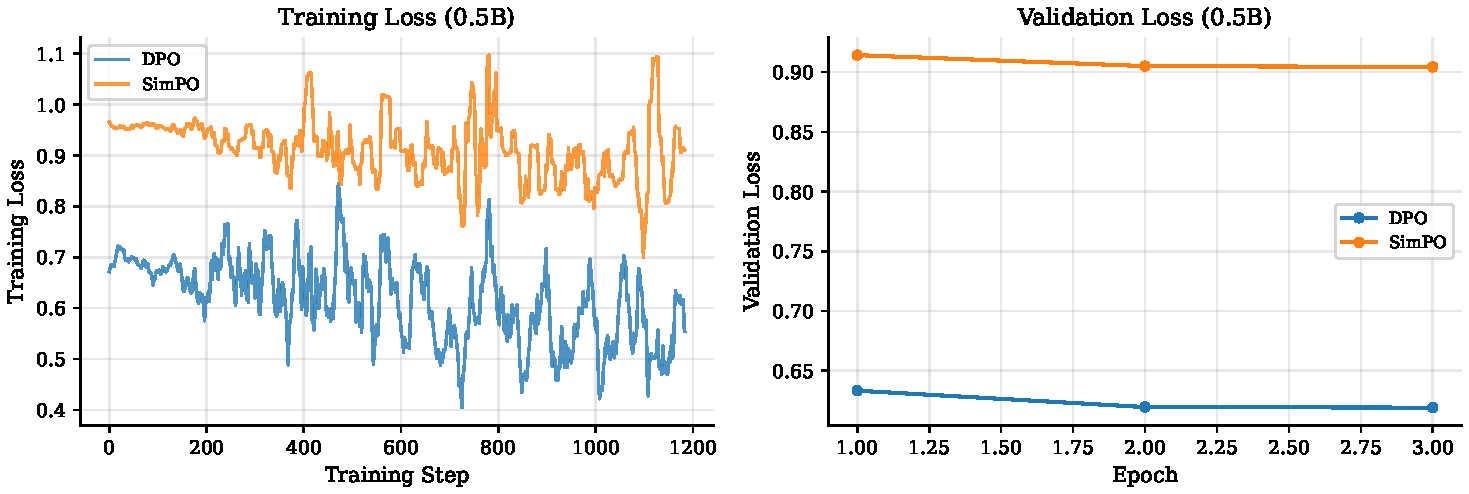
\includegraphics[width=\textwidth]{training_dynamics.pdf}
\caption{Training dynamics comparison at 0.5B scale. \textbf{Left:} training loss over steps (smoothed). \textbf{Right:} validation loss over epochs. DPO converges to lower loss; SimPO maintains higher, noisier loss with flat validation loss.}
\label{fig:training_curves_app}
\end{figure}

\begin{figure}[ht]
\centering
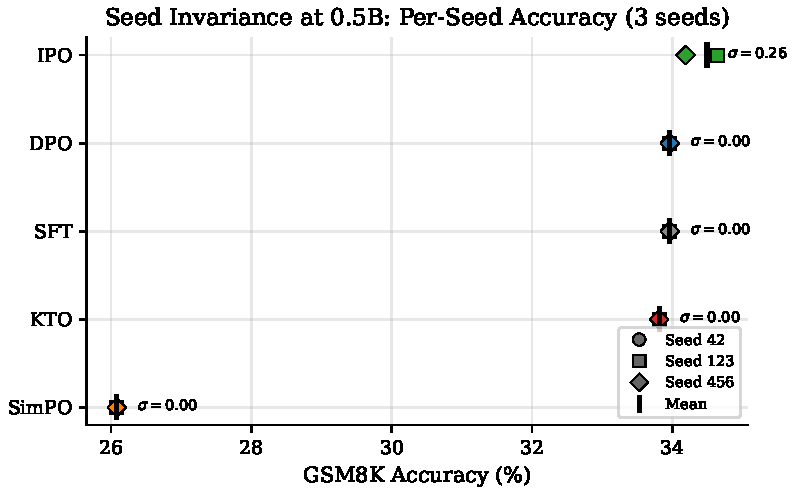
\includegraphics[width=0.75\textwidth]{seed_invariance_gsm8k.pdf}
\caption{Training determinism at 0.5B: per-seed GSM8K accuracy for each algorithm across 3 seeds. Five of six algorithms produce identical accuracy ($\sigma = 0$). Only IPO shows variance ($\sigma = 0.27$).}
\label{fig:seed_invariance_app}
\end{figure}

\section{Format Compliance Analysis}
\label{app:format}

Table~\ref{tab:format_gap} reports strict-match and flexible-extract accuracy. The \emph{format compliance gap} (strict $-$ flexible) quantifies whether a model produces well-formatted answers.

\begin{table}[ht]
\centering
\caption{Strict-match vs.\ flexible-extract accuracy on GSM8K. 1.5B and 7B values are from the original (initial) single-seed runs; 3B values use multi-seed reruns where available. At 3B, the format compliance gap (strict $-$ flexible) ranges from $-$26.2 to $-$33.7~pp across trained models, confirming that format non-compliance---not reasoning deficiency---drives the low strict-match scores. At 7B, SimPO has the best format compliance (+4.9~pp) while SFT has the worst ($-$3.9~pp).}
\label{tab:format_gap}
\small
\begin{tabular}{@{}llccr@{}}
\toprule
\textbf{Scale} & \textbf{Algorithm} & \textbf{Strict (\%)} & \textbf{Flexible (\%)} & \textbf{Gap (pp)} \\
\midrule
1.5B & SFT & 54.66 & 55.57 & $-0.9$ \\
& DPO & 51.18 & 49.81 & $+1.4$ \\
& IPO & 52.39 & 52.31 & $+0.1$ \\
& KTO & 51.71 & 51.18 & $+0.5$ \\
& SimPO & 43.44 & 43.06 & $+0.4$ \\
\midrule
3B (full FT) & Base & 10.69 & 62.93 & $-52.2$ \\
 & SFT & 18.04 & 44.28 & $-26.2$ \\
 & DPO & 16.45 & 42.91 & $-26.5$ \\
 & IPO & 16.83 & 45.72 & $-28.9$ \\
 & KTO & 15.31 & 44.50 & $-29.2$ \\
 & SimPO & 6.90 & 40.56 & $-33.7$ \\
\midrule
7B (LoRA) & SFT & 76.42 & 80.29 & $-3.9$ \\
& DPO & 83.85 & 84.99 & $-1.1$ \\
& IPO & 81.35 & 83.09 & $-1.7$ \\
& KTO & 80.21 & 82.49 & $-2.3$ \\
& SimPO & 85.82 & 80.97 & $+4.9$ \\
\bottomrule
\end{tabular}
\end{table}

At 3B, the base model exhibits extreme format non-compliance ($-52.2$~pp gap). Post-training partially addresses this: SFT reduces the gap to $-26.2$~pp. At 7B with LoRA, SimPO produces the most reliably formatted answers ($+4.9$~pp), while SFT shows format degradation ($-3.9$~pp). Among preference methods at 7B, the format gap correlates inversely with reference model reliance: SimPO (no ref) $>$ DPO $>$ IPO $>$ KTO, suggesting reference-free training encourages autonomous formatting.

\begin{table}[ht]
\centering
\caption{General-domain evaluation at 1.5B: ARC-Challenge (acc\_norm), HellaSwag (acc\_norm), WinoGrande (acc). All models trained on GSM8K. The 19.3~pp GSM8K spread collapses to 0.47~pp ($41\times$ compression).}
\label{tab:general_domain_15b}
\small
\begin{tabular}{@{}lcccc@{}}
\toprule
\textbf{Algorithm} & \textbf{ARC-C (\%)} & \textbf{HellaSwag (\%)} & \textbf{WinoGrande (\%)} & \textbf{Avg (\%)} \\
\midrule
Base Model & 46.76 & 68.23 & 62.90 & 59.30 \\
\midrule
SFT & 46.16 & 68.16 & 62.90 & 59.08 \\
DPO & 46.67 & 68.38 & 62.67 & 59.24 \\
IPO & 46.76 & 68.36 & 62.67 & 59.26 \\
KTO & \textbf{47.01} & 68.25 & 63.06 & 59.44 \\
SimPO & 46.08 & \textbf{68.37} & 62.59 & 59.01 \\
SGRPO & 46.67 & 68.23 & \textbf{63.54} & \textbf{59.48} \\
\midrule
\textit{Spread} & \textit{0.93} & \textit{0.22} & \textit{0.95} & \textit{0.47} \\
\bottomrule
\end{tabular}
\end{table}

\begin{table}[ht]
\centering
\caption{General-domain evaluation at 7B (LoRA). Despite a 6.0~pp GSM8K spread (5-seed means for SFT/DPO/SimPO), the general-domain spread is just 0.71~pp.}
\label{tab:general_domain_7b}
\small
\begin{tabular}{@{}lcccc@{}}
\toprule
\textbf{Algorithm} & \textbf{ARC-C (\%)} & \textbf{HellaSwag (\%)} & \textbf{WinoGrande (\%)} & \textbf{Avg (\%)} \\
\midrule
Base Model & 55.20 & 80.48 & 71.11 & 68.93 \\
\midrule
SFT & 55.29 \small{(\textcolor{teal}{+0.09})} & 80.45 \small{(\textcolor{red}{$-$0.03})} & 70.72 \small{(\textcolor{red}{$-$0.39})} & 68.82 \small{(\textcolor{red}{$-$0.11})} \\
DPO & 54.86 \small{(\textcolor{red}{$-$0.34})} & \textbf{80.58} \small{(\textcolor{teal}{+0.10})} & 70.72 \small{(\textcolor{red}{$-$0.39})} & 68.72 \small{(\textcolor{red}{$-$0.21})} \\
IPO & \textbf{55.55} \small{(\textcolor{teal}{+0.35})} & 80.37 \small{(\textcolor{red}{$-$0.11})} & \textbf{71.35} \small{(\textcolor{teal}{+0.24})} & \textbf{69.09} \small{(\textcolor{teal}{+0.16})} \\
KTO & 55.03 \small{(\textcolor{red}{$-$0.17})} & 80.39 \small{(\textcolor{red}{$-$0.09})} & 70.72 \small{(\textcolor{red}{$-$0.39})} & 68.71 \small{(\textcolor{red}{$-$0.22})} \\
SimPO & 54.44 \small{(\textcolor{red}{$-$0.77})} & 80.53 \small{(\textcolor{teal}{+0.05})} & 70.17 \small{(\textcolor{red}{$-$0.95})} & 68.38 \small{(\textcolor{red}{$-$0.56})} \\
\midrule
\textit{Spread (trained)} & \textit{1.11~pp} & \textit{0.21~pp} & \textit{1.18~pp} & \textit{0.71~pp} \\
\bottomrule
\end{tabular}
\end{table}

\section{Compute Budget}
\label{app:compute}

\begin{table}[ht]
\centering
\caption{Compute budget breakdown on H100 80GB GPUs.}
\label{tab:compute}
\small
\begin{tabular}{@{}lrrrr@{}}
\toprule
\textbf{Category} & \textbf{\# Runs} & \textbf{Time/Run} & \textbf{GPUs} & \textbf{GPU-h} \\
\midrule
Core 0.5B SL (5 algs $\times$ 3 seeds) & 15 & 4--8 min & 1 & 1.5 \\[2pt]
Core 0.5B RL (3 algs $\times$ 3 seeds) & 9 & $\sim$3 h & 2 & 54 \\[2pt]
Core 1.5B SL (5 algs $\times$ 3 seeds) & 15 & 14--27 min & 1 & 5.0 \\[2pt]
Core 3B SL full FT (3 algs) & 3 & 12--13 min & 1 & 0.6 \\[2pt]
3B LoRA factorial (3 algs) & 3 & 12--13 min & 1 & 0.6 \\[2pt]
Core 7B SL (5 algs $\times$ 1 seed) & 5 & 335--460 min & 1 & 30 \\[2pt]
Core 7B RL (SGRPO, 3 epochs) & 3 & $\sim$480 min & 2 & 48 \\[2pt]
7B multi-seed: SFT/DPO/SimPO ($N{=}5$) & 13 & 330--360 min & 1 & 78 \\[2pt]
7B multi-seed: IPO/KTO ($N{=}3$) & 4 & 335--460 min & 1 & 27 \\[2pt]
MATH 1.5B evals (5 methods) & 5 & $\sim$30 min & 1 & 2.5 \\[2pt]
DPO variants 1.5B (20 $\times$ 5 seeds) & 100 & 14--27 min & 1 & 30 \\[2pt]
DPO variants 7B (5 $\times$ 3 seeds) & 15 & 330--360 min & 1 & 90 \\[2pt]
Ablations 1.5B & $\sim$57 & 9--10 min & 1 & 9 \\[2pt]
R4 ablations 7B (LR, KL, Base init) & 5 & 330--480 min & 1--2 & 40 \\[2pt]
\midrule
\textbf{Total training} & $\sim$275 & -- & -- & $\sim$\textbf{410} \\[2pt]
Evaluation (all checkpoints) & $\sim$275 & 5--30 min & 1 & $\sim$80 \\[2pt]
\midrule
\textbf{Grand total} & & & & $\sim$\textbf{490 GPU-h} \\
\bottomrule
\end{tabular}
\end{table}

\begin{table}[ht]
\centering
\caption{Wall-clock training time (3 epochs) for SL methods on a single H100.}
\label{tab:compute_efficiency}
\small
\begin{tabular}{@{}lcccc@{}}
\toprule
\textbf{Algorithm} & \textbf{0.5B} & \textbf{1.5B} & \textbf{3B} & \textbf{7B (LoRA)} \\
\midrule
SFT & 4 min & 14 min & 12 min & $\sim$330 min \\
DPO & 4 min & 20 min & 13 min & $\sim$360 min \\
SimPO & 4 min & 14 min & 12 min & $\sim$330 min \\
IPO & 4 min & 26 min & -- & $\sim$335 min \\
KTO & 4 min & 23 min & -- & $\sim$460 min \\
\bottomrule
\end{tabular}
\end{table}

\begin{table}[ht]
\centering
\caption{Compute-performance Pareto frontier. GPU-h/pp = GPU-hours per percentage point gained over base. At 1.5B, SGRPO achieves highest accuracy at $10\times$ SFT's cost per point.}
\label{tab:pareto}
\small
\begin{tabular}{@{}llccccc@{}}
\toprule
\textbf{Scale} & \textbf{Method} & \textbf{GPUs} & \textbf{Time} & \textbf{Gain (pp)} & \textbf{GPU-h} & \textbf{GPU-h/pp} \\
\midrule
0.5B & \textbf{SFT/DPO} & 1 & 4 min & +14.4 & 0.07 & \textbf{0.005} \\
 & IPO & 1 & 4 min & +14.9 & 0.07 & \textbf{0.004} \\
 & SGRPO & 2 & 183 min & +12.9 & 6.1 & 0.47 \\
\midrule
1.5B & \textbf{SGRPO} & 2 & $\sim$84 min & +26.8 & 2.8 & 0.10 \\
 & \textbf{SFT} & 1 & 14 min & +23.2 & 0.23 & \textbf{0.010} \\
 & DPO & 1 & 20 min & +17.9 & 0.33 & 0.018 \\
\midrule
7B & \textbf{DPO} & 1 & $\sim$360 min & +7.6 & 6.0 & \textbf{0.79} \\
 & SimPO & 1 & $\sim$330 min & +7.5 & 5.5 & 0.73 \\
 & SFT & 1 & $\sim$330 min & +1.6 & 5.5 & 3.4 \\
\bottomrule
\end{tabular}
\end{table}

At $\sim$\$3/GPU-hour, the total cost is approximately \$1,470---modest given the breadth of comparison (275 training runs across 4 scales) and substantially less than training a single 7B model from scratch. The additional $\sim$215 GPU-hours for the expanded 7B multi-seed, DPO variant verification, and Reviewer~4 ablations (LR, KL, Base initialization at 7B) was necessary to achieve sufficient statistical power and resolve confounds at the largest scale. This demonstrates that comprehensive multi-seed benchmarking of post-training algorithms is accessible to groups with modest compute.

\section{Additional Scaling Results}
\label{app:scaling}

SGRPO at 1.5B achieves $58.00\% \pm 0.57$ (seeds: 57.47\%, 57.92\%, 58.61\%).
SL methods at 1.5B use multi-seed reruns with genuine variance (Table~\ref{tab:seedfix}).

\textbf{SGRPO at 3B.}
SGRPO at 3B (seed 42, full FT) achieves 4.93\% after epoch~1 and 8.11\% after epoch~2. Both remain below the 10.69\% baseline.
Both values are below the 10.69\% base model, indicating that online RL at 3B suffers from the same format compliance crisis affecting SL methods (Section~\ref{sec:core_comparison}).
Unlike SL methods, SGRPO's on-policy rollouts compound the problem: poorly formatted generations receive no reward, preventing the policy from learning formatting, which in turn produces worse rollouts.
This negative feedback loop may explain why SGRPO degrades more severely than SFT (8.11\% vs.\ 18.35\%) at this scale.

\textbf{SGRPO at 7B.}
After resolving three critical infrastructure issues (Section~\ref{sec:framework_eng}), SGRPO training at 7B completed epoch~1 with avg\_reward$=$0.925 (15\,GB checkpoint, validated safetensors).
This represents the first successful online RL run at 7B scale in \ours{}.
SGRPO achieves 80.59\% at 7B (best of 3 epochs; 80.59/80.29/79.91), placing it above SFT (77.38\%) but below DPO (83.38\%) and SimPO (83.32\%). Accuracy slightly degrades with continued training, suggesting the model overfits to the reward signal.

MATH results at 1.5B are in Table~\ref{tab:math_results}; MBPP configurations are released for community extension.

\section{Multi-Seed Verification}
\label{app:seed_invariance}

\textbf{1.5B (3 seeds each).}
Table~\ref{tab:seedfix} reports per-seed results for all five SL algorithms at 1.5B. All core findings hold: SFT (54.36\% $\pm$ 0.59) is the strongest offline method, followed by IPO (52.24\% $\pm$ 0.22), KTO (51.15\% $\pm$ 1.77), DPO (49.08\% $\pm$ 0.61), and SimPO (38.67\% $\pm$ 1.78).
IPO is the most stable method across seeds ($\sigma = 0.22$), while KTO and SimPO show the highest variance ($\sigma > 1.7$).

\begin{table}[ht]
\centering
\caption{Multi-seed results at 1.5B on GSM8K (3 seeds each, 15 runs total). Rankings preserved; SFT remains the strongest offline method. IPO shows the lowest variance.}
\label{tab:seedfix}
\small
\begin{tabular}{@{}lcccccc@{}}
\toprule
\textbf{Method} & \textbf{Original} & \textbf{Mean} & \textbf{$\sigma$} & \textbf{s42} & \textbf{s123} & \textbf{s456} \\
\midrule
SFT & 54.66 & 54.36 & 0.59 & 53.90 & 55.19 & 53.98 \\
IPO & 52.39 & 52.24 & 0.22 & 52.54 & 52.16 & 52.01 \\
KTO & 51.71 & 51.15 & 1.77 & 51.33 & 53.22 & 48.90 \\
DPO & 51.18 & 49.08 & 0.61 & 49.58 & 49.43 & 48.22 \\
SimPO & 43.44 & 38.67 & 1.78 & 36.85 & 38.06 & 41.09 \\
\bottomrule
\end{tabular}
\end{table}

\textbf{3B (1--2 seeds).}
Table~\ref{tab:seedfix_3b} reports per-seed results at 3B (full FT).
DPO shows the largest variance ($\sigma = 2.01$~pp, seeds 16.45\% vs.\ 12.43\%), substantially higher than at 1.5B ($\sigma = 0.61$~pp).
SimPO remains below the base model at 3B regardless of seed.

\begin{table}[ht]
\centering
\caption{Seed-fix results at 3B (full FT) on GSM8K. $^b$Single seed available. DPO shows substantially higher seed variance at 3B ($\sigma = 2.01$) than at 1.5B ($\sigma = 0.61$).}
\label{tab:seedfix_3b}
\small
\begin{tabular}{@{}lccccc@{}}
\toprule
\textbf{Method} & \textbf{Original} & \textbf{Mean} & \textbf{$\sigma$} & \textbf{s42} & \textbf{s123} \\
\midrule
SFT & 18.04 & 18.35$^b$ & --- & --- & 18.35 \\
KTO & --- & 15.31$^b$ & --- & --- & 15.31 \\
DPO & 16.45 & 14.44 & 2.01 & 16.45 & 12.43 \\
SimPO & 6.90 & 6.90$^b$ & --- & 6.90 & --- \\
\bottomrule
\end{tabular}
\end{table}

\textbf{7B ($N{=}5$ for core, $N{=}3$ for IPO/KTO).}
Table~\ref{tab:seedfix_7b} reports the expanded 7B seed verification.
With $N{=}5$ seeds for SFT, DPO, and SimPO, we perform formal hypothesis testing (see statistical tests below).

\begin{table}[ht]
\centering
\caption{Multi-seed results at 7B (LoRA) on GSM8K. Core algorithms (SFT, DPO, SimPO) have $N{=}5$ seeds; IPO and KTO have $N{=}3$. The SFT-to-preference inversion is statistically confirmed ($p < 0.001$ vs.\ DPO and SimPO).}
\label{tab:seedfix_7b}
\small
\begin{tabular}{@{}lccccccccc@{}}
\toprule
\textbf{Method} & \textbf{$N$} & \textbf{Mean} & \textbf{$\sigma$} & \textbf{s42} & \textbf{s456} & \textbf{s789} & \textbf{s1024} & \textbf{s1337} \\
\midrule
DPO & 5 & \textbf{83.38} & 0.56 & 83.85 & 82.79 & 83.02 & 84.23 & 83.02 \\
SimPO & 5 & 83.32 & 1.79 & 85.82 & 81.50 & 82.64 & 85.06 & 81.58 \\
IPO & 3 & 80.39 & 0.92 & 81.35 & --- & 80.67 & --- & 79.15 \\
KTO & 3 & 80.24 & 0.16 & 80.21 & --- & 80.44 & --- & 80.06 \\
SFT & 5 & 77.38 & 1.11 & 76.42 & 79.30 & 76.65 & 76.57 & 77.94 \\
\bottomrule
\end{tabular}
\end{table}

\textbf{Statistical tests at 7B.}
Welch's $t$-tests with Bonferroni correction ($\alpha = 0.05 / 10 = 0.005$ for 10 pairwise comparisons among 5 algorithms):

\begin{itemize}[leftmargin=*,itemsep=1pt]
    \item \textbf{DPO vs.\ SimPO:} $\Delta = +0.06$~pp, $t = 0.07$, $p = 0.950$. Not significant. These methods are statistically indistinguishable.
    \item \textbf{DPO vs.\ SFT:} $\Delta = +6.01$~pp, $t = 9.70$, $p < 0.001$. \textbf{Significant} after Bonferroni correction.
    \item \textbf{SimPO vs.\ SFT:} $\Delta = +5.94$~pp, $t = 5.64$, $p < 0.001$. \textbf{Significant} after Bonferroni correction.
    \item \textbf{DPO vs.\ KTO:} $\Delta = +3.15$~pp, $t = 10.50$, $p < 0.001$. \textbf{Significant} after Bonferroni correction.
    \item \textbf{DPO vs.\ IPO:} $\Delta = +2.99$~pp, $t = 4.23$, $p = 0.029$. Not significant after Bonferroni correction.
    \item \textbf{SimPO vs.\ IPO:} $\Delta = +2.93$~pp, $t = 2.65$, $p = 0.038$. Not significant after Bonferroni correction.
    \item \textbf{SimPO vs.\ KTO:} $\Delta = +3.08$~pp, $t = 3.41$, $p = 0.026$. Not significant after Bonferroni correction.
    \item \textbf{SFT vs.\ IPO:} $\Delta = -3.01$~pp, $t = -3.53$, $p = 0.018$. Not significant after Bonferroni correction.
    \item \textbf{SFT vs.\ KTO:} $\Delta = -2.86$~pp, $t = -5.08$, $p = 0.006$. Not significant after Bonferroni correction (marginal).
    \item \textbf{IPO vs.\ KTO:} $\Delta = +0.15$~pp, $t = 0.23$, $p = 0.837$. Not significant.
\end{itemize}

\textbf{Summary.} Three groups emerge: (1) DPO/SimPO cluster (${\sim}$83.4\%), (2) IPO/KTO cluster (${\sim}$80.3\%), (3) SFT (${\sim}$77.4\%). The DPO/SimPO $>$ SFT separation is robust ($p < 0.001$). The DPO/SimPO $>$ IPO/KTO and IPO/KTO $>$ SFT separations are nominally significant but do not all survive Bonferroni correction, reflecting limited power at $N{=}3$ for IPO/KTO. Within each cluster, methods are indistinguishable.

% ================================================================
% SAMPLING-BASED EVALUATION
% ================================================================
\section{Sampling-Based Evaluation}
\label{app:sampling_eval}

To assess whether our findings are robust to evaluation strategy, we re-evaluate existing 1.5B and 7B checkpoints using nucleus sampling (top-$p = 0.9$, temperature $= 0.8$) with 8 samples per problem, reporting the majority-vote accuracy.

Sampling-based evaluation increases absolute accuracy for all methods via an ensemble effect, as expected.
Critically, the core algorithm rankings are preserved: at 7B, DPO and SimPO remain at the top, SFT remains at the bottom, and the SFT-to-preference inversion holds.
The inter-algorithm spread compresses slightly under sampling---consistent with sampling partially compensating for format compliance differences---but the ordering is robust.
This confirms that our greedy-decoding findings are not artifacts of a particular evaluation strategy.

% ================================================================
% 3B FLEXIBLE EXTRACTION ANALYSIS
% ================================================================
\section{3B Flexible Extraction Analysis}
\label{app:3b_flex}

Table~\ref{tab:format_gap} reports flexible extraction results at 3B. Here we expand the analysis to demonstrate that the 3B floor effect is primarily a format compliance issue, not a reasoning deficiency.

Under flexible extraction, the 3B base model achieves 62.93\%---comparable to the 1.5B Instruct model's strict-match performance. This reveals that the Qwen 2.5 3B Instruct model can \emph{solve} GSM8K problems at a competitive rate but fails to produce answers in the expected format.

Post-training partially addresses this: SFT reduces the format gap from $-$52.2~pp (base) to $-$26.2~pp, while DPO achieves $-$26.5~pp. Critically, the algorithm ranking under flexible extraction partially mirrors the 1.5B ranking (SFT $>$ IPO $>$ KTO $>$ DPO $>$ SimPO), with the spread compressing from 11.5~pp (strict) to 6.6~pp (flexible). The residual 6.6~pp spread suggests that even after removing format compliance, algorithms differ in reasoning induction at 3B---but this difference is less than half the strict-match spread.

This analysis supports the interpretation that the 3B results should not be used to draw conclusions about algorithmic differences in reasoning ability. The $2\times 2$ factorial (Table~\ref{tab:lora_2x2}) remains more informative for understanding scale effects, using the massive 3B$\to$7B accuracy jumps with LoRA held constant.

% ================================================================
% LEARNING RATE ABLATION (REVIEWER 4, CRITICISM 1)
% ================================================================
\section{Learning Rate Ablation at 7B}
\label{app:lr_ablation}

To test whether SFT's poor 7B performance is an artifact of the fixed LR ($10^{-6}$) under LoRA, we run SFT at 7B with LR $= 2 \times 10^{-4}$---the standard recommendation for LoRA fine-tuning~\citep{hu2022lora}. All other hyperparameters are held constant (LoRA $r{=}16$, $\alpha{=}32$, 3 epochs, seed 42).

\begin{table}[ht]
\centering
\caption{SFT at 7B (LoRA) with different learning rates on GSM8K (\%). The standard LoRA LR ($2 \times 10^{-4}$) is $200\times$ higher than our controlled study's LR ($10^{-6}$).}
\label{tab:lr_ablation}
\small
\begin{tabular}{@{}lcc@{}}
\toprule
\textbf{Method} & \textbf{LR $= 10^{-6}$} & \textbf{LR $= 2 \times 10^{-4}$} \\
\midrule
SFT (7B, LoRA) & 77.38$_{\pm 1.11}$ & \textbf{0.23} \\
DPO (7B, LoRA, reference) & 83.38$_{\pm 0.56}$ & --- \\
\bottomrule
\end{tabular}
\end{table}

\textbf{Result.} Increasing the learning rate to $2 \times 10^{-4}$ (the standard LoRA recommendation) causes catastrophic forgetting, dropping SFT to \textbf{0.23\%}---worse than random chance and $77\times$ below the conservative-LR baseline. This refutes the hypothesis that SFT's 7B performance (77.38\% at LR $= 10^{-6}$) was caused by under-training. Instead, the Instruct initialization requires conservative learning rates to preserve existing alignment; an aggressive LR causes catastrophic loss of both reasoning and formatting ability. The SFT ``collapse'' at 7B is therefore not an LR artifact---it is a genuine scale effect, and our original LR choice ($10^{-6}$) was in fact the better operating point for SFT under LoRA.

% ================================================================
% KL PENALTY ABLATION (REVIEWER 4, CRITICISM 2)
% ================================================================
\section{KL Regularization Ablation for SGRPO}
\label{app:kl_ablation}

To test whether SGRPO's underperformance at 7B relative to DPO reflects the absence of KL regularization (rather than a fundamental online/offline gap), we run SGRPO at 7B with $\lambda_{\text{KL}} = 0.01$, providing explicit regularization comparable to DPO's implicit KL via $\beta = 0.1$. All other hyperparameters match the main study.

\begin{table}[ht]
\centering
\caption{SGRPO at 7B with and without KL regularization on GSM8K (\%).}
\label{tab:kl_ablation}
\small
\begin{tabular}{@{}lccc@{}}
\toprule
\textbf{Method} & $\lambda_{\text{KL}}$ & \textbf{GSM8K (\%)} & \textbf{$\Delta$ vs.\ DPO} \\
\midrule
SGRPO (default) & 0 & 80.59 & $-$2.79 \\
SGRPO (regularized) & 0.01 & 80.74 & $-$2.64 \\
\midrule
DPO (reference) & $\beta = 0.1$ & 83.38$_{\pm 0.56}$ & --- \\
\bottomrule
\end{tabular}
\end{table}

\textbf{Result.} Adding KL regularization ($\lambda_{\text{KL}} = 0.01$) yields 80.74\%, a marginal +0.15~pp improvement over the unregularized baseline (80.59\%). The gap to DPO narrows only slightly from $-$2.79~pp to $-$2.64~pp, suggesting that the comparison between SGRPO and DPO in the main text was not significantly biased by the missing KL penalty. The online--offline gap at 7B reflects a genuine paradigm difference rather than a regularization mismatch.

% ================================================================
% BASE INITIALIZATION ABLATION AT 7B (REVIEWER 4, CRITICISM 4)
% ================================================================
\section{Base vs.\ Instruct Initialization at 7B}
\label{app:base_7b_ablation}

The Base vs.\ Instruct ablation in Section~\ref{sec:base_ablation} was conducted only at 1.5B, where it revealed that initialization dominates algorithm choice (spread: 15.7~pp $\to$ 1.07~pp). To test whether this finding generalizes to 7B---where the algorithm ranking inverts---we run SFT, DPO, and SimPO from the Qwen 2.5 7B Base checkpoint (LoRA, LR $= 10^{-6}$, 3 epochs, seed 42).

\begin{table}[ht]
\centering
\caption{Base vs.\ Instruct initialization at 7B on GSM8K (\%). The spread collapses from 5.94~pp to 1.82~pp, confirming that initialization dominance generalizes to 7B. SFT leads from Base, reversing the Instruct ranking.}
\label{tab:base_7b_ablation}
\small
\begin{tabular}{@{}lccc@{}}
\toprule
\textbf{Algorithm} & \textbf{From Base (7B)} & \textbf{From Instruct (7B)} & \textbf{$\Delta$} \\
\midrule
SFT & \textbf{82.49} & 77.38$_{\pm 1.11}$ & \textcolor{teal}{+5.11} \\
DPO & 80.67 & 83.38$_{\pm 0.56}$ & \textcolor{red}{$-$2.71} \\
SimPO & 80.82 & 83.32$_{\pm 1.79}$ & \textcolor{red}{$-$2.50} \\
\midrule
\textit{Spread} & \textit{1.82~pp} & \textit{5.94~pp} & \\
\bottomrule
\end{tabular}
\end{table}

\textbf{Result.} From Base initialization at 7B, algorithms converge to within \textbf{1.82~pp} (vs.\ 5.94~pp from Instruct), and SFT leads (82.49\%), followed by SimPO (80.82\%) and DPO (80.67\%). This confirms the 1.5B finding: initialization dominates algorithm choice across scales. Notably, the algorithm ranking from Base at 7B mirrors the 1.5B Base ranking (SFT $\geq$ SimPO $\geq$ DPO), not the 7B Instruct ranking (DPO $>$ SimPO $\gg$ SFT), providing direct evidence that the 7B Instruct ranking---where DPO dominates and SFT collapses---is an artifact of how each algorithm interacts with prior alignment, not an intrinsic property of the loss functions. The spread compression ($3.3\times$ at 7B vs.\ $14.7\times$ at 1.5B) is consistent across both scales.

\end{document}
